\documentclass[12pt]{article}

% Packages
\usepackage[margin=2.5cm]{geometry}
\usepackage{amsmath}
\usepackage{amssymb}
\usepackage{bm}
\usepackage{graphicx}
\usepackage{physics}
\usepackage{tikz}
\usetikzlibrary{arrows.meta, positioning, shapes.geometric}

% Better boxes
\usepackage{amsfonts}

% No indentation
\setlength{\parindent}{0pt}
\setlength{\parskip}{6pt}

\begin{document}

	\title{Guidelines for Adsorption Isotherm Models}
	\maketitle

	\tableofcontents
	\newpage

	\section{Langmuir isotherm}
	
	The Langmuir isotherm is usually written as
	\begin{equation}
		q_e = \frac{Q_{\max} K_L C_e}{1 + K_L C_e},
		\label{eq:Langmuir}
	\end{equation}
	where \(q_e\) is the equilibrium adsorbed amount, \(C_e\) is the equilibrium
	concentration in the fluid phase, \(Q_{\max}\) is the maximum adsorption
	capacity, and \(K_L\) is the Langmuir equilibrium constant.
	
	\subsection{High concentration limit, $Q_{max}$: \(C_e \to \infty\)}
	
	From eq.~\eqref{eq:Langmuir},
	\begin{equation}
		\lim_{C_e \to \infty} q_e
		= \lim_{C_e \to \infty}
		\frac{Q_{\max} K_L C_e}{1 + K_L C_e}.
	\end{equation}
	Dividing numerator and denominator by \(K_L C_e\) gives
	\begin{equation}
		\lim_{C_e \to \infty} q_e
		= Q_{\max} \lim_{C_e \to \infty}
		\frac{1}{\frac{1}{K_L C_e} + 1}
		%= Q_{\max} \cdot \frac{1}{0 + 1}
		= Q_{\max}.
	\end{equation}
	Therefore, the Langmuir isotherm saturates at
	\begin{equation}
		\boxed{\displaystyle \lim_{C_e \to \infty} q_e = Q_{\max}}.
	\end{equation}
	
	\subsection{Low concentration limit: Henry constant as the initial slope}
	
	For small \(C_e\), such that \(K_L C_e \ll 1\), the denominator of
	eq.~\eqref{eq:Langmuir} can be expanded:
	\begin{equation}
		\frac{1}{1 + K_L C_e} \approx 1 - K_L C_e + \mathcal{O}(C_e^2).
	\end{equation}
	Substituting into eq.~\eqref{eq:Langmuir} and keeping only the first order
	term in \(C_e\),
	\begin{equation}
		q_e \approx Q_{\max} K_L C_e.
	\end{equation}
	The Henry law form is
	\begin{equation}
		q_e \approx K_H C_e,
	\end{equation}
	so that the Henry constant is identified as the initial slope at
	\(C_e \to 0\):
	\begin{equation}
		K_H = \left.\frac{\mathrm{d}q_e}{\mathrm{d}C_e}\right|_{C_e \to 0}
		= Q_{\max} K_L.
	\end{equation}
	Thus,
	\begin{equation}
		\boxed{K_H = Q_{\max} K_L.}
	\end{equation}
	
	\subsection{Adsorption free energy}
	
	The Langmuir constant \(K_L\) is an equilibrium constant that can be
	related to the standard Gibbs free energy of adsorption. To make the
	constant dimensionless, one introduces a standard concentration
	\(C^0\) (typically \(1~\mathrm{mol~L^{-1}}\)) and defines
	\begin{equation}
		K_L^{\ast} = K_L C^0.
	\end{equation}
	The standard Gibbs free energy of adsorption is then
	\begin{equation}
		\Delta G_{\mathrm{ads}}^{0}
		= - R T \ln K_L^{\ast}
		= - R T \ln\left( K_L C^0 \right),
	\end{equation}
	where \(R\) is the gas constant and \(T\) is the absolute temperature.
	
	An adsorption affinity energy \(E_{\mathrm{aff}}\) can be naturally defined
	as the magnitude of this free energy:
	\begin{equation}
		E_{\mathrm{aff}} = - \Delta G_{\mathrm{ads}}^{0}
		= R T \ln\left( K_L C^0 \right).
	\end{equation}
	Therefore, the Langmuir constant provides a direct connection between
	the macroscopic isotherm parameters and the microscopic thermodynamic
	driving force for adsorption:
	\begin{equation}
		\boxed{\Delta G_{\mathrm{ads}}^{0}
			= - R T \ln\left( K_L C^0 \right),
			\qquad
			E_{\mathrm{aff}} = R T \ln\left( K_L C^0 \right).}
	\end{equation}
	
	\subsection{Energy distribution as a function of temperature}
	
	For a single Langmuir site, the adsorption affinity energy is
	\begin{equation}
		E_{\mathrm{aff}}(T)
		= R T \ln\!\left(K_L C^0\right),
		\label{eq:Eaff_def}
	\end{equation}
	where \(K_L\) is the Langmuir equilibrium constant, \(C^0\) is a standard
	concentration, \(R\) is the gas constant, and \(T\) is the absolute
	temperature.
	
	In a heterogeneous adsorbent, one can consider a continuous distribution of
	Langmuir constants \(K_L\), characterized by a normalized distribution
	function \(g(K_L)\),
	\begin{equation}
		\int_{0}^{\infty} g(K_L)\, \mathrm{d}K_L = 1.
	\end{equation}
	Using eq.~\eqref{eq:Eaff_def}, the energy and the equilibrium constant are
	related by
	\begin{equation}
		E = R T \ln\!\left(K_L C^0\right),
		\qquad
		K_L = \frac{1}{C^0} \exp\!\left(\frac{E}{R T}\right).
		\label{eq:K_of_E}
	\end{equation}
	
	The corresponding distribution of adsorption energies, \(f(E;T)\), is
	obtained by a change of variables,
	\begin{equation}
		f(E;T)\, \mathrm{d}E = g(K_L)\, \mathrm{d}K_L.
	\end{equation}
	Using eq.~\eqref{eq:K_of_E}, one has
	\begin{equation}
		\frac{\mathrm{d}K_L}{\mathrm{d}E}
		= \frac{1}{C^0} \frac{1}{R T}
		\exp\!\left(\frac{E}{R T}\right)
		= \frac{K_L(E,T)}{R T},
	\end{equation}
	so that
	\begin{equation}
		f(E;T)
		= g\!\left(K_L(E,T)\right)
		\frac{\mathrm{d}K_L}{\mathrm{d}E}
		= g\!\left(\frac{1}{C^0} \exp\!\frac{E}{R T}\right)
		\frac{1}{R T C^0}
		\exp\!\left(\frac{E}{R T}\right).
		\label{eq:f_E_T_general}
	\end{equation}
	
	Equation~\eqref{eq:f_E_T_general} shows explicitly how the energy
	distribution \(f(E;T)\) depends on temperature through both the exponential
	factor and the mapping \(K_L(E,T)\). If the intrinsic heterogeneity of the
	surface is represented by a temperature-independent distribution \(g(K_L)\),
	the apparent energy distribution observed in adsorption experiments still
	changes with \(T\) because higher-energy sites are progressively weighted by
	the Boltzmann-type factor \(\exp(E / R T)\).
	
	
	\begin{figure}
		\centering
		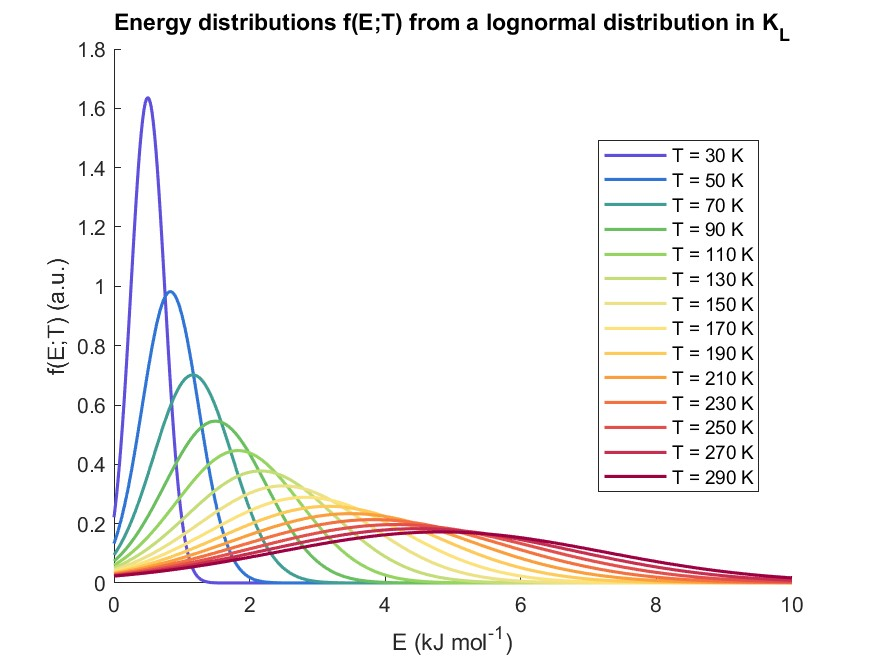
\includegraphics[width=0.75\linewidth]{Langmuir_energy.jpg}
		\caption{Energy distribution in function of energy for Langmuir isotherm}
		\label{fig:Langmuir_energy}
	\end{figure}
	
	\section{Double Langmuir}
	
	% Dual-site (Double) Langmuir isotherm: limits and Henry-law behavior
	
	The dual-site (double) Langmuir isotherm can be written as
	\begin{equation}
		q_e
		= \frac{Q_{\max,1} K_1 C_e}{1 + K_1 C_e}
		+ \frac{Q_{\max,2} K_2 C_e}{1 + K_2 C_e},
		\label{eq:DoubleLangmuir}
	\end{equation}
	where \(q_e\) is the equilibrium adsorbed amount, \(C_e\) is the
	equilibrium concentration in the fluid phase, \(Q_{\max,i}\) is the
	maximum adsorption capacity of site \(i\), and \(K_i\) is the Langmuir
	equilibrium constant for site \(i\) (with \(i = 1,2\)).
	
	\subsection{High concentration limit: \(C_e \to \infty\)}
	
	Consider the limit \(C_e \to \infty\) in eq.~\eqref{eq:DoubleLangmuir}.
	For each site,
	\begin{equation}
		\lim_{C_e \to \infty} \frac{Q_{\max,i} K_i C_e}{1 + K_i C_e}
		= Q_{\max,i} \lim_{C_e \to \infty}
		\frac{K_i C_e}{1 + K_i C_e}.
	\end{equation}
	Dividing numerator and denominator by \(K_i C_e\) gives
	\begin{equation}
		\lim_{C_e \to \infty} \frac{Q_{\max,i} K_i C_e}{1 + K_i C_e}
		= Q_{\max,i} \lim_{C_e \to \infty}
		\frac{1}{\frac{1}{K_i C_e} + 1}
		= Q_{\max,i} \cdot \frac{1}{0 + 1}
		= Q_{\max,i}.
	\end{equation}
	Therefore, the total loading at saturation is
	\begin{equation}
		\lim_{C_e \to \infty} q_e
		= Q_{\max,1} + Q_{\max,2}.
	\end{equation}
	Defining the total maximum capacity
	\begin{equation}
		Q_{\max}^{\mathrm{(tot)}} = Q_{\max,1} + Q_{\max,2},
	\end{equation}
	we obtain
	\begin{equation}
		\boxed{\displaystyle \lim_{C_e \to \infty} q_e
			= Q_{\max}^{\mathrm{(tot)}}.}
	\end{equation}
	
	\subsection{Low concentration limit: global Henry constant at \(C_e \to 0\)}
	
	For small \(C_e\), such that \(K_i C_e \ll 1\) for both sites,
	we can expand each term in eq.~\eqref{eq:DoubleLangmuir}:
	\begin{equation}
		\frac{1}{1 + K_i C_e}
		\approx 1 - K_i C_e + \mathcal{O}(C_e^2).
	\end{equation}
	Substituting this into eq.~\eqref{eq:DoubleLangmuir} and keeping only
	the first-order terms in \(C_e\),
	\begin{align}
		q_e
		&\approx Q_{\max,1} K_1 C_e (1 - K_1 C_e)
		+ Q_{\max,2} K_2 C_e (1 - K_2 C_e) \\
		&\approx Q_{\max,1} K_1 C_e + Q_{\max,2} K_2 C_e,
	\end{align}
	where second-order terms in \(C_e\) have been neglected.
	
	This has the form of Henry law,
	\begin{equation}
		q_e \approx K_H^{\mathrm{(tot)}} C_e,
	\end{equation}
	with the global Henry constant given by the initial slope at
	\(C_e \to 0\):
	\begin{equation}
		K_H^{\mathrm{(tot)}}
		= \left.\frac{\mathrm{d} q_e}{\mathrm{d} C_e}\right|_{C_e \to 0}
		= Q_{\max,1} K_1 + Q_{\max,2} K_2.
	\end{equation}
	It is convenient to define the Henry constant of each site as
	\begin{equation}
		K_{H,1} = Q_{\max,1} K_1,
		\qquad
		K_{H,2} = Q_{\max,2} K_2,
	\end{equation}
	so that
	\begin{equation}
		\boxed{K_H^{\mathrm{(tot)}} = K_{H,1} + K_{H,2}
			= Q_{\max,1} K_1 + Q_{\max,2} K_2.}
	\end{equation}
	Thus, the dual-site Langmuir isotherm recovers Henry-law behavior at
	low concentration, with a total Henry constant equal to the sum of
	the site-specific Henry contributions.
	
	\subsection{Effective Langmuir constant for the dual-site model}
	
	For a single-site Langmuir isotherm, the Henry constant and the
	Langmuir constant are related by
	\begin{equation}
		K_H = Q_{\max} K_L.
	\end{equation}
	It is therefore natural, for the dual-site Langmuir model, to define
	an effective total maximum capacity
	\begin{equation}
		Q_{\max}^{\mathrm{(tot)}} = Q_{\max,1} + Q_{\max,2},
	\end{equation}
	and a formal effective Langmuir constant \(K_L^{\mathrm{(tot)}}\)
	such that, at low concentration, the isotherm can be written in the
	single-site form
	\begin{equation}
		q_e \approx Q_{\max}^{\mathrm{(tot)}} K_L^{\mathrm{(tot)}} C_e
		\qquad (C_e \to 0).
	\end{equation}
	Comparing this expression with the Henry-law form
	\begin{equation}
		q_e \approx K_H^{\mathrm{(tot)}} C_e,
	\end{equation}
	and using
	\begin{equation}
		K_H^{\mathrm{(tot)}} = Q_{\max,1} K_1 + Q_{\max,2} K_2,
	\end{equation}
	we obtain
	\begin{equation}
		K_H^{\mathrm{(tot)}} = Q_{\max}^{\mathrm{(tot)}} K_L^{\mathrm{(tot)}}.
	\end{equation}
	Hence, the effective Langmuir constant for the dual-site model is
	\begin{equation}
		K_L^{\mathrm{(tot)}}
		= \frac{K_H^{\mathrm{(tot)}}}{Q_{\max}^{\mathrm{(tot)}}}
		= \frac{Q_{\max,1} K_1 + Q_{\max,2} K_2}
		{Q_{\max,1} + Q_{\max,2}}.
	\end{equation}
	This shows that \(K_L^{\mathrm{(tot)}}\) is a capacity-weighted
	average of the site-specific Langmuir constants:
	\begin{equation}
		\boxed{
			K_L^{\mathrm{(tot)}}
			= \frac{Q_{\max,1}}{Q_{\max,1} + Q_{\max,2}} K_1
			+ \frac{Q_{\max,2}}{Q_{\max,1} + Q_{\max,2}} K_2.
		}
	\end{equation}
	
	\subsection{Thermodynamic interpretation of the effective Langmuir constant}
	
	As in the single-site case, the (dimensionful) Langmuir constants
	\(K_1\), \(K_2\), and \(K_L^{\mathrm{(tot)}}\) can be converted into
	dimensionless equilibrium constants by introducing a standard state
	concentration \(C^0\) (typically \(1~\mathrm{mol~L^{-1}}\)):
	\begin{equation}
		K_i^{\ast} = K_i C^0,
		\qquad
		K_L^{\mathrm{(tot)}\ast} = K_L^{\mathrm{(tot)}} C^0.
	\end{equation}
	The corresponding standard Gibbs free energies of adsorption for
	each site and for the effective dual-site description are then
	\begin{equation}
		\Delta G_{\mathrm{ads},i}^{0}
		= - R T \ln K_i^{\ast}
		= - R T \ln\left( K_i C^0 \right),
	\end{equation}
	and
	\begin{equation}
		\Delta G_{\mathrm{ads}}^{0,\mathrm{(tot)}}
		= - R T \ln K_L^{\mathrm{(tot)}\ast}
		= - R T \ln\left( K_L^{\mathrm{(tot)}} C^0 \right).
	\end{equation}
	An effective adsorption affinity energy associated with the dual-site
	isotherm can be defined as the magnitude of this free energy:
	\begin{equation}
		E_{\mathrm{aff}}^{\mathrm{(tot)}}
		= - \Delta G_{\mathrm{ads}}^{0,\mathrm{(tot)}}
		= R T \ln\left( K_L^{\mathrm{(tot)}} C^0 \right).
	\end{equation}
	In this sense, the dual-site Langmuir model can be mapped onto a
	single effective Langmuir isotherm that reproduces both the total
	saturation capacity \(Q_{\max}^{\mathrm{(tot)}}\) and the initial
	Henry-law slope \(K_H^{\mathrm{(tot)}}\), while the microscopic
	heterogeneity between sites is encoded in the capacity-weighted
	average that defines \(K_L^{\mathrm{(tot)}}\).
	
	\subsection{From Langmuir to heterogeneous isotherms via site-energy distributions}

	The key idea behind several classical isotherm models is that a
	heterogeneous surface can be described as a collection of independent
	Langmuir sites, each characterized by an adsorption energy~$E$.
	The overall isotherm is then the integral of local Langmuir
	contributions weighted by the site-energy distribution~$f(E)$:
	\begin{equation}
		q_e = Q_{\max} \int_{0}^{\infty}
		\frac{K(E)\, C_e}{1 + K(E)\, C_e}\, f(E)\, \mathrm{d}E,
		\label{eq:general_heterogeneous}
	\end{equation}
	where $K(E) = K_0 \exp(E / RT)$ is the local Langmuir constant
	associated with energy~$E$, $K_0$ is a pre-exponential factor,
	$R$ is the gas constant, and $T$ is the absolute temperature.

	Different choices of $f(E)$ lead to different macroscopic isotherms,
	as summarized in Fig.~\ref{fig:isotherm_family_tree}.

	\begin{figure}[p]
		\centering
		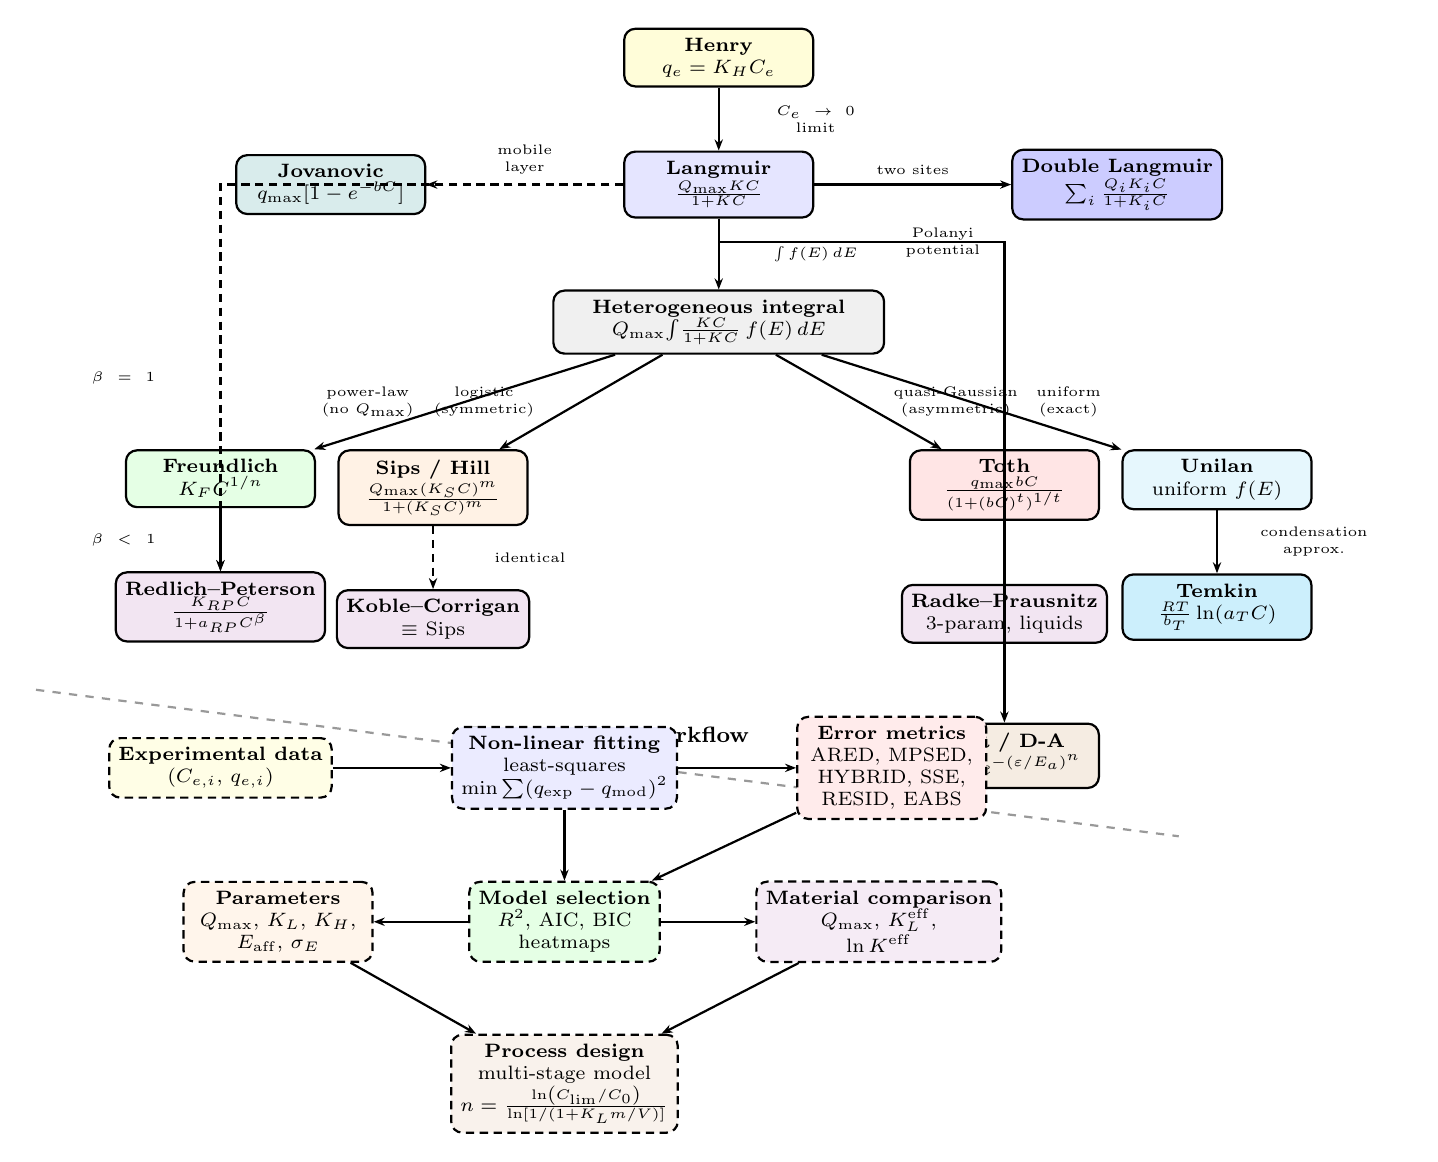
\begin{tikzpicture}[
			every node/.style={font=\scriptsize},
			box/.style={draw, rounded corners, minimum width=2.4cm,
				minimum height=0.7cm, align=center, thick},
			databox/.style={draw, rounded corners, minimum width=2.4cm,
				minimum height=0.7cm, align=center, thick,
				densely dashed},
			arr/.style={-{Stealth[length=4pt]}, thick},
			darr/.style={-{Stealth[length=4pt]}, thick, densely dashed},
			note/.style={font=\tiny, text width=2.2cm, align=center},
			sep/.style={draw=black!40, thick, dashed},
			]
			% =============================================================
			%  PART A: MODEL FAMILY (left half)
			% =============================================================
			% --- Henry ---
			\node[box, fill=yellow!15] (henry)
			{\textbf{Henry}\\$q_e = K_H C_e$};

			% --- Langmuir ---
			\node[box, fill=blue!10, below=0.8cm of henry] (lang)
			{\textbf{Langmuir}\\$\frac{Q_{\max}KC}{1+KC}$};

			% --- Double Langmuir ---
			\node[box, fill=blue!20, right=2.5cm of lang] (dlang)
			{\textbf{Double Langmuir}\\$\sum_i\frac{Q_i K_i C}{1+K_i C}$};

			% --- Jovanovic (different kernel) ---
			\node[box, fill=teal!15, left=2.5cm of lang] (jov)
			{\textbf{Jovanovic}\\$q_{\max}[1-e^{-bC}]$};

			% --- General heterogeneous integral ---
			\node[box, fill=gray!12, below=0.9cm of lang,
			minimum width=4.2cm] (het)
			{\textbf{Heterogeneous integral}\\
				$Q_{\max}\!\int\!\frac{KC}{1+KC}\,f(E)\,dE$};

			% --- Energy-distribution models (Row 1) ---
			\node[box, fill=green!10,
			below left=1.2cm and 3.0cm of het] (freund)
			{\textbf{Freundlich}\\$K_F C^{1/n}$};
			\node[box, fill=orange!10,
			below left=1.2cm and 0.3cm of het] (sips)
			{\textbf{Sips / Hill}\\$\frac{Q_{\max}(K_SC)^m}{1+(K_SC)^m}$};
			\node[box, fill=red!10,
			below right=1.2cm and 0.3cm of het] (toth)
			{\textbf{Toth}\\$\frac{q_{\max}bC}{(1+(bC)^t)^{1/t}}$};
			\node[box, fill=cyan!10,
			below right=1.2cm and 3.0cm of het] (unilan)
			{\textbf{Unilan}\\uniform $f(E)$};

			% --- Temkin (condensation approx of Unilan) ---
			\node[box, fill=cyan!20, below=0.8cm of unilan] (temkin)
			{\textbf{Temkin}\\$\frac{RT}{b_T}\ln(a_T C)$};

			% --- Three-parameter bridges (Row 2) ---
			\node[box, fill=violet!10, below=0.8cm of freund] (rp)
			{\textbf{Redlich--Peterson}\\$\frac{K_{RP}C}{1+a_{RP}C^\beta}$};
			\node[box, fill=violet!10, below=0.8cm of sips] (kc)
			{\textbf{Koble--Corrigan}\\$\equiv$ Sips};
			\node[box, fill=violet!10, below=0.8cm of toth] (radke)
			{\textbf{Radke--Prausnitz}\\3-param, liquids};

			% --- Micropore models ---
			\node[box, fill=brown!15, below=1.0cm of radke] (da)
			{\textbf{D-R / D-A}\\$Q_{\max}e^{-(\varepsilon/E_a)^n}$};

			% ---- ARROWS: model relationships ----
			\draw[arr] (henry) -- (lang)
			node[midway, right, note] {$C_e\to 0$\\limit};
			\draw[arr] (lang) -- (dlang)
			node[midway, above, note] {two sites};
			\draw[darr] (lang) -- (jov)
			node[midway, above, note] {mobile\\layer};
			\draw[arr] (lang) -- (het)
			node[midway, right, note] {$\int f(E)\,dE$};
			\draw[arr] (het) -- (freund)
			node[midway, left, note] {power-law\\(no $Q_{\max}$)};
			\draw[arr] (het) -- (sips)
			node[midway, left, note] {logistic\\(symmetric)};
			\draw[arr] (het) -- (toth)
			node[midway, right, note] {quasi-Gaussian\\(asymmetric)};
			\draw[arr] (het) -- (unilan)
			node[midway, right, note] {uniform\\(exact)};
			\draw[arr] (unilan) -- (temkin)
			node[midway, right, note] {condensation\\approx.};
			\draw[darr] (freund) -- (rp)
			node[midway, left, note] {$\beta<1$};
			\draw[darr] (lang) -| (rp)
			node[near end, left, note] {$\beta=1$};
			\draw[darr] (sips) -- (kc)
			node[midway, right, note] {identical};
			\draw[arr] (lang.south) -- ++(0,-0.3) -| (da.north)
			node[near start, right, note, text width=1.8cm]
			{Polanyi\\potential};

			% =============================================================
			%  PART B: DATA HANDLING WORKFLOW (bottom)
			% =============================================================
			% Separator line
			\coordinate (sepl) at ([yshift=-0.6cm]rp.south west);
			\coordinate (sepr) at ([yshift=-0.6cm]da.south east);
			\draw[sep] ([xshift=-1cm]sepl) -- ([xshift=1cm]sepr)
			node[midway, above=2pt, font=\footnotesize\bfseries]
			{Data handling workflow};

			% --- Experimental data ---
			\node[databox, fill=yellow!10,
			below=1.2cm of rp] (expdata)
			{\textbf{Experimental data}\\$(C_{e,i},\, q_{e,i})$};

			% --- Non-linear fitting ---
			\node[databox, fill=blue!8,
			right=1.5cm of expdata] (nlfit)
			{\textbf{Non-linear fitting}\\least-squares\\$\min\sum(q_{\exp}-q_{\mathrm{mod}})^2$};

			% --- Error metrics ---
			\node[databox, fill=red!8,
			right=1.5cm of nlfit] (errors)
			{\textbf{Error metrics}\\ARED, MPSED,\\HYBRID, SSE,\\RESID, EABS};

			% --- Model selection ---
			\node[databox, fill=green!10,
			below=0.9cm of nlfit] (select)
			{\textbf{Model selection}\\$R^2$, AIC, BIC\\heatmaps};

			% --- Parameter extraction ---
			\node[databox, fill=orange!8,
			left=1.2cm of select] (params)
			{\textbf{Parameters}\\$Q_{\max}$, $K_L$, $K_H$,\\$E_{\mathrm{aff}}$, $\sigma_E$};

			% --- Material comparison ---
			\node[databox, fill=violet!8,
			right=1.2cm of select] (compare)
			{\textbf{Material comparison}\\$Q_{\max}$, $K_L^{\mathrm{eff}}$,\\$\ln K^{\mathrm{eff}}$};

			% --- Design ---
			\node[databox, fill=brown!10,
			below=0.9cm of select] (design)
			{\textbf{Process design}\\multi-stage model\\$n = \frac{\ln(C_{\lim}/C_0)}%
				{\ln[1/(1+K_L m/V)]}$};

			% ---- ARROWS: workflow ----
			\draw[arr] (expdata) -- (nlfit);
			\draw[arr] (nlfit) -- (errors);
			\draw[arr] (errors) -- (select);
			\draw[arr] (nlfit) -- (select);
			\draw[arr] (select) -- (params);
			\draw[arr] (select) -- (compare);
			\draw[arr] (params) -- (design);
			\draw[arr] (compare) -- (design);
		\end{tikzpicture}
		\caption{Complete overview: (top)~family of adsorption isotherm
			models and their interrelationships --- solid arrows denote
			formal derivations, dashed arrows denote limiting-case or
			empirical connections; (bottom)~data handling workflow from
			experimental measurements to process design.}
		\label{fig:isotherm_family_tree}
	\end{figure}

	\subsubsection{Derivation of the Freundlich isotherm}

	If the energy distribution follows a power law,
	\begin{equation}
		f(E) = \frac{n}{\pi}\sin(\pi n)\,
		K_0^{\,n}\, \mathrm{e}^{\,nE/RT},
		\qquad 0 < n < 1,
	\end{equation}
	the substitution $y = K(E)\,C_e$ in Eq.~\eqref{eq:general_heterogeneous}
	leads to an integral of the form
	\begin{equation}
		q_e \propto C_e^{\,n}
		\int_{C_e K_0}^{\infty} \frac{y^{-n}}{1 + y}\,\mathrm{d}y.
		\label{eq:freundlich_derivation_step}
	\end{equation}
	In the regime $C_e K_0 \ll 1$, one may extend the lower limit from
	$C_e K_0$ to~$0$ and quantify the incurred error. Indeed,
	\begin{equation}
		\int_{C_e K_0}^{\infty} \frac{y^{-n}}{1+y}\, \mathrm{d}y
		=
		\int_{0}^{\infty} \frac{y^{-n}}{1+y}\, \mathrm{d}y
		-
		\int_{0}^{C_e K_0} \frac{y^{-n}}{1+y}\, \mathrm{d}y,
	\end{equation}
	and the remainder satisfies
	\begin{equation}
		0 \le \int_{0}^{C_e K_0} \frac{y^{-n}}{1+y}\, \mathrm{d}y
		\le \frac{(C_e K_0)^{1-n}}{1-n},
		\qquad 0<n<1,
	\end{equation}
	so the approximation becomes asymptotically exact as $C_e K_0 \to 0$.
	The constant integral is evaluated by the change of variables
	$y = t/(1-t)$, giving
	\begin{align}
		\int_{0}^{\infty} \frac{y^{-n}}{1+y}\, \mathrm{d}y
		&= \int_{0}^{1} t^{(1-n)-1}(1-t)^{n-1}\, \mathrm{d}t
		= B(1-n,\,n) \nonumber\\
		&= \Gamma(1-n)\,\Gamma(n),
		\label{eq:beta_integral_gamma}
	\end{align}
	and Euler's reflection formula $\Gamma(n)\Gamma(1-n) = \pi/\sin(\pi n)$
	yields
	\begin{equation}
		\int_{0}^{\infty} \frac{y^{-n}}{1+y}\, \mathrm{d}y
		= \frac{\pi}{\sin(\pi n)}, \qquad 0<n<1,
		\label{eq:beta_integral}
	\end{equation}
	which leads directly to the Freundlich form
	$q_e = K_F C_e^{1/n}$ (Eq.~\eqref{eq:Freundlich}),
	with $K_F$ absorbing all prefactors. Because the power-law distribution
	is unbounded, no finite $Q_{\max}$ emerges.

	\subsubsection{Derivation of the Sips isotherm}

	If the site-energy distribution is a \emph{logistic} (symmetric)
	density with location~$E_c$ and scale $b = nRT$,
	\begin{equation}
		f(E) = \frac{1}{b}\,
		\frac{\exp\!\bigl(\frac{E - E_c}{b}\bigr)}
		{\Bigl[1 + \exp\!\bigl(\frac{E - E_c}{b}\bigr)\Bigr]^{2}},
		\label{eq:sips_energy_dist}
	\end{equation}
	substitution into Eq.~\eqref{eq:general_heterogeneous} and evaluation
	within the condensation approximation yields
	\begin{equation}
		q_e = \frac{Q_{\max}\,(K_S C_e)^{m}}{1 + (K_S C_e)^{m}},
		\label{eq:Sips_derived}
	\end{equation}
	where $m = 1/n$ is the heterogeneity exponent and
	$K_S = K_0\exp(E_c / RT)$.
	The logistic distribution is symmetric about~$E_c$, so the Sips
	isotherm describes surfaces whose site energies are symmetrically
	distributed around a mean value.
	When $m = 1$ (i.e.\ $n = 1$, zero heterogeneity), the distribution
	collapses to a Dirac delta and Eq.~\eqref{eq:Sips_derived} reduces
	to the single-site Langmuir isotherm.

	\subsubsection{Derivation of the Toth isotherm}

	The Toth isotherm arises when the energy distribution is a
	\emph{quasi-Gaussian, asymmetric} density skewed toward low
	energies. Although no simple closed-form expression for $f(E)$
	exists in this case, the resulting macroscopic isotherm can be
	written as
	\begin{equation}
		q_e = q_{\max}\,
		\frac{b\,C_e}{\bigl[1 + (b\,C_e)^{t}\bigr]^{1/t}},
		\label{eq:Toth_derived}
	\end{equation}
	where $t$ is the heterogeneity parameter ($0 < t \leq 1$) and
	$b$ is an affinity constant. The asymmetry of $f(E)$ distinguishes
	the Toth model from the Sips model: the energy distribution has a
	longer tail toward low adsorption energies, making it more suitable
	for surfaces where the majority of sites are weaker than the mean.
	When $t = 1$, the distribution becomes symmetric and
	Eq.~\eqref{eq:Toth_derived} reduces to the Langmuir isotherm.

	\subsubsection{Derivation of the Temkin isotherm}

	In the condensation approximation, sites with energy $E$ such that
	$K(E)\,C_e \gg 1$ are fully occupied, while sites with
	$K(E)\,C_e \ll 1$ are empty. The critical energy at which
	$K(E_c)\,C_e = 1$ is
	\begin{equation}
		E_c(C_e) = -RT\ln(K_0 C_e).
		\label{eq:temkin_Ec}
	\end{equation}
	If the energy distribution is \emph{uniform} over a finite band
	$[E_{\min},\, E_{\max}]$,
	\begin{equation}
		f(E) = \frac{1}{E_{\max} - E_{\min}},
		\qquad E_{\min} \leq E \leq E_{\max},
		\label{eq:temkin_fE}
	\end{equation}
	the total coverage in the condensation limit is proportional to the
	fraction of sites that are filled:
	\begin{equation}
		q_e \approx Q_{\max}\,
		\frac{E_{\max} - E_c(C_e)}{E_{\max} - E_{\min}}.
	\end{equation}
	Substituting Eq.~\eqref{eq:temkin_Ec},
	\begin{align}
		q_e
		&\approx Q_{\max}\,
		\frac{E_{\max} + RT\ln(K_0 C_e)}{E_{\max} - E_{\min}}
		\nonumber\\
		&= \frac{Q_{\max}\,RT}{E_{\max} - E_{\min}}
		\ln\!\left(K_0\, \mathrm{e}^{E_{\max}/RT}\, C_e\right).
	\end{align}
	Defining
	\begin{equation}
		\frac{RT}{b_T} = \frac{Q_{\max}\,RT}{E_{\max} - E_{\min}},
		\qquad
		a_T = K_0\, \mathrm{e}^{E_{\max}/RT},
	\end{equation}
	one recovers the Temkin isotherm
	\begin{equation}
		\boxed{q_e = \frac{RT}{b_T}\,\ln(a_T C_e).}
	\end{equation}
	The Temkin model is therefore valid only in the intermediate range
	$E_{\min} < E_c(C_e) < E_{\max}$; outside this range the
	condensation approximation breaks down, which explains why the
	Temkin equation is unphysical at both $C_e \to 0$ and
	$C_e \to \infty$.

	\subsubsection{Derivation of the Unilan isotherm}

	The Unilan model also uses a uniform (rectangular) energy
	distribution, but retains the exact local Langmuir kernel instead
	of the condensation approximation. Writing
	\begin{equation}
		f(E) = \frac{1}{2s}, \qquad E_c - s \leq E \leq E_c + s,
		\label{eq:unilan_fE}
	\end{equation}
	and substituting into Eq.~\eqref{eq:general_heterogeneous},
	\begin{equation}
		q_e = \frac{Q_{\max}}{2s}
		\int_{E_c - s}^{E_c + s}
		\frac{K_0\,\mathrm{e}^{E/RT}\, C_e}
		{1 + K_0\,\mathrm{e}^{E/RT}\, C_e}\,\mathrm{d}E.
	\end{equation}
	With the substitution $u = K_0\,\mathrm{e}^{E/RT}\,C_e$, so that
	$\mathrm{d}E = RT\,\mathrm{d}u / u$, the integral becomes
	\begin{equation}
		q_e = \frac{Q_{\max}}{2s}\, RT
		\int_{u_{\min}}^{u_{\max}}
		\frac{1}{1 + u}\,\frac{\mathrm{d}u}{u}
		\cdot u \cdot \frac{1}{u},
	\end{equation}
	which after simplification evaluates to
	\begin{equation}
		q_e = \frac{Q_{\max}\,RT}{2s}
		\ln\!\left(
		\frac{1 + K_0\,\mathrm{e}^{(E_c+s)/RT}\,C_e}
		{1 + K_0\,\mathrm{e}^{(E_c-s)/RT}\,C_e}
		\right).
		\label{eq:Unilan_derived}
	\end{equation}
	Defining $b_{\max} = K_0\,\mathrm{e}^{(E_c+s)/RT}$ and
	$b_{\min} = K_0\,\mathrm{e}^{(E_c-s)/RT}$, this can be written as
	\begin{equation}
		\boxed{q_e = \frac{Q_{\max}\,RT}{2s}
		\ln\!\left(
		\frac{1 + b_{\max}\, C_e}{1 + b_{\min}\, C_e}
		\right).}
	\end{equation}
	When $s \to 0$ (homogeneous surface), $b_{\max} \to b_{\min} = K_L$
	and l'H\^opital's rule recovers the single-site Langmuir isotherm.
	Notice that the Temkin and Unilan models share the same uniform
	$f(E)$, but differ in the treatment of the local isotherm: Temkin
	uses the condensation (step-function) approximation, while Unilan
	retains the full Langmuir kernel.

	\subsubsection{Derivation of the Jovanovic isotherm}

	The Jovanovic model does not arise from a particular energy
	distribution inserted into the Langmuir kernel of
	Eq.~\eqref{eq:general_heterogeneous}. Instead, it uses a different
	\emph{local isotherm}. Whereas Langmuir assumes immobile, localised
	adsorption with no lateral interactions, Jovanovic's statistical
	mechanical treatment of a mobile adsorbed layer yields the local
	coverage
	\begin{equation}
		\theta_{\mathrm{Jov}}(E, C_e)
		= 1 - \exp\!\bigl(-K(E)\,C_e\bigr),
		\label{eq:jovanovic_local}
	\end{equation}
	with $K(E) = K_0\,\mathrm{e}^{E/RT}$ as before. The homogeneous
	(single-energy) Jovanovic isotherm is therefore
	\begin{equation}
		\boxed{q_e = q_{\max}\bigl[1 - \exp(-b\,C_e)\bigr],}
	\end{equation}
	with $b = K_0\,\mathrm{e}^{E_0/RT}$. Generalisation to a
	heterogeneous surface proceeds by replacing the Langmuir kernel in
	Eq.~\eqref{eq:general_heterogeneous} with
	Eq.~\eqref{eq:jovanovic_local}:
	\begin{equation}
		q_e = Q_{\max}\int_{0}^{\infty}
		\bigl[1 - \exp(-K(E)\,C_e)\bigr]\, f(E)\,\mathrm{d}E.
		\label{eq:jovanovic_het}
	\end{equation}
	Choosing a logistic $f(E)$ as in the Sips case
	(Eq.~\eqref{eq:sips_energy_dist}) and applying the condensation
	approximation to Eq.~\eqref{eq:jovanovic_het} yields the
	\emph{Jovanovic--Freundlich} isotherm
	\begin{equation}
		q_e = Q_{\max}\bigl[1 - \exp\!\bigl(-(K_S C_e)^m\bigr)\bigr],
	\end{equation}
	which reduces to the simple Jovanovic form when $m = 1$.

	\subsubsection{Derivation of the Redlich--Peterson isotherm}

	The Redlich--Peterson model can be understood as a Langmuir-type
	expression in which the denominator is modified to include a
	Freundlich-type nonlinearity. Starting from the general form
	\begin{equation}
		q_e = \frac{K_{RP}\, C_e}{1 + a_{RP}\, C_e^{\,\beta}},
	\end{equation}
	this does not correspond to a single well-defined energy
	distribution $f(E)$ in Eq.~\eqref{eq:general_heterogeneous}.
	Rather, it can be motivated as an \emph{interpolation}:
	\begin{itemize}
		\item At low $C_e$: $a_{RP}\,C_e^{\beta} \ll 1$, so
		$q_e \approx K_{RP}\,C_e$ (Henry law).
		\item At high $C_e$: $q_e \approx (K_{RP}/a_{RP})\,
		C_e^{1-\beta}$ (Freundlich-type power law).
		\item When $\beta = 1$: exact Langmuir form.
	\end{itemize}
	The model thus provides a three-parameter empirical bridge between
	Langmuir (correct low-$C_e$ limit with finite $K_H$) and Freundlich
	(heterogeneous high-$C_e$ regime), without requiring an explicit
	energy distribution.

	\subsubsection{Koble--Corrigan: equivalence with Sips}

	The Koble--Corrigan isotherm,
	\begin{equation}
		q_e = \frac{A_{KC}\, C_e^{\,1/n}}{1 + B_{KC}\, C_e^{\,1/n}},
	\end{equation}
	is algebraically identical to the Sips isotherm
	(Eq.~\eqref{eq:Sips_derived}) under the identifications
	$Q_{\max} = A_{KC}/B_{KC}$, $K_S = B_{KC}$, and $m = 1/n$.
	Its derivation from the heterogeneous integral via the logistic
	energy distribution is therefore the same as for Sips.

	\subsubsection{Radke--Prausnitz: empirical construction}

	The Radke--Prausnitz isotherm,
	\begin{equation}
		q_e = \frac{a_{RP}\, r_{RP}\, C_e}
		{a_{RP} + r_{RP}\, C_e^{\,p-1}},
	\end{equation}
	was constructed empirically to simultaneously satisfy:
	\begin{itemize}
		\item Henry law at low $C_e$: $q_e \approx r_{RP}\,C_e$.
		\item Freundlich-type behavior at high $C_e$:
		$q_e \approx a_{RP}\, C_e^{\,2-p}$.
	\end{itemize}
	No closed-form energy distribution $f(E)$ is known for this model.
	It is best regarded as a flexible empirical interpolation designed
	for liquid-phase adsorption data.

	\subsubsection{Dubinin--Radushkevich and Dubinin--Astakhov:
		Polanyi potential theory}

	The D-R and D-A models do not originate from the heterogeneous
	Langmuir integral (Eq.~\eqref{eq:general_heterogeneous}) but from
	a fundamentally different framework: the \emph{Polanyi adsorption
	potential theory}. The central concept is the adsorption potential
	\begin{equation}
		\varepsilon = RT\ln\!\left(1 + \frac{1}{C_e/C_s}\right),
		\label{eq:polanyi_potential}
	\end{equation}
	where $C_s$ is the saturation concentration.
	The theory postulates that the volume filled in the micropore
	follows a \emph{characteristic curve} that depends only on
	$\varepsilon$:
	\begin{equation}
		\frac{q_e}{Q_{\max}}
		= \exp\!\left[-\left(\frac{\varepsilon}{E_a}\right)^{n_{DA}}
		\right].
		\label{eq:DA_derived}
	\end{equation}
	The D-R model is the special case $n_{DA} = 2$ (Gaussian energy
	distribution in the micropore), while $n_{DA} \neq 2$ accounts for
	broader or narrower pore-size distributions.

	Although conceptually distinct from the site-energy integral
	approach, an approximate connection exists: if one defines a
	Gaussian-like distribution of adsorption energies
	\begin{equation}
		f(E) \propto \exp\!\left[-\left(\frac{E - E_0}{E_a}\right)^{n_{DA}}
		\right],
	\end{equation}
	and applies the condensation approximation to
	Eq.~\eqref{eq:general_heterogeneous}, the D-A form
	(Eq.~\eqref{eq:DA_derived}) is recovered. Thus, D-R/D-A can be
	viewed as condensation-approximation isotherms with a
	(generalised) Gaussian energy distribution, specific to
	microporous adsorbents.

	\subsubsection{Hill isotherm: cooperativity from Sips}

	The Hill isotherm
	\begin{equation}
		q_e = Q_{\max}\,\frac{C_e^{\,n_H}}{K_D + C_e^{\,n_H}}
	\end{equation}
	is mathematically identical to the Sips model with the
	substitutions $m = n_H$ and $K_S = K_D^{-1/n_H}$ (see
	Eq.~\eqref{eq:Sips_derived}). Its derivation from the
	heterogeneous integral is therefore the same logistic
	$f(E)$ as for Sips.

	The key difference is physical: while the Sips exponent $m < 1$
	represents \emph{surface heterogeneity} (broad energy
	distribution), the Hill coefficient $n_H > 1$ represents
	\emph{positive cooperativity} (binding of one molecule enhances
	the affinity for the next). When $n_H > 1$, the isotherm is
	sigmoidal (S-shaped), a feature that cannot arise from
	heterogeneity alone ($m \leq 1$ always gives a concave
	isotherm).

	\section{Freundlich isotherm}
	
	The Freundlich isotherm is an empirical model commonly written as
	\begin{equation}
		q_e = K_F C_e^{1/n},
		\label{eq:Freundlich}
	\end{equation}
	where \(q_e\) is the equilibrium adsorbed amount, \(C_e\) is the
	equilibrium concentration in the fluid phase, \(K_F\) is the
	Freundlich constant related to adsorption capacity, and \(1/n\)
	is a heterogeneity parameter (typically \(0 < 1/n < 1\)).
	
	\subsection{High concentration limit: absence of an intrinsic \(Q_{\max}\)}
	
	In contrast to the Langmuir isotherm, the Freundlich model does not
	contain a built-in saturation capacity. Taking the limit of
	eq.~\eqref{eq:Freundlich} for large \(C_e\),
	\begin{equation}
		\lim_{C_e \to \infty} q_e
		= \lim_{C_e \to \infty} K_F C_e^{1/n}.
	\end{equation}
	For any fixed \(K_F > 0\) and \(1/n > 0\), we have
	\begin{equation}
		\lim_{C_e \to \infty} C_e^{1/n} = \infty,
	\end{equation}
	so that
	\begin{equation}
		\lim_{C_e \to \infty} q_e = \infty.
	\end{equation}
	Therefore, the Freundlich isotherm does not predict a finite
	saturation capacity:
	\begin{equation}
		\boxed{
			\text{Freundlich has no intrinsic } Q_{\max};
			\quad
			\lim_{C_e \to \infty} q_e = \infty.
		}
	\end{equation}
	
	In practical applications, one sometimes introduces an
	\emph{effective} or \emph{operational} saturation capacity by
	restricting the validity of the Freundlich model to a maximum
	concentration \(C_{\max}\) (for example, the upper limit of the
	experimental range). In that case, an effective capacity may be
	defined as
	\begin{equation}
		Q_{\max}^{\mathrm{(F,eff)}} = q_e(C_{\max})
		= K_F C_{\max}^{1/n},
	\end{equation}
	which should be understood as a phenomenological quantity, not
	a true thermodynamic saturation.
	
	\subsection{Low concentration behavior: comparison with Henry law}
	
	Henry law for dilute solutions is written as
	\begin{equation}
		q_e \approx K_H C_e,
		\label{eq:Henry}
	\end{equation}
	with \(K_H\) the Henry constant, equal to the initial slope of the
	isotherm at \(C_e \to 0\):
	\begin{equation}
		K_H = \left. \frac{\mathrm{d} q_e}{\mathrm{d} C_e}\right|_{C_e \to 0}.
	\end{equation}
	
	For the Freundlich isotherm, the derivative of \(q_e\) is
	\begin{equation}
		\frac{\mathrm{d} q_e}{\mathrm{d} C_e}
		= K_F \frac{1}{n} C_e^{1/n - 1}.
	\end{equation}
	Taking the limit as \(C_e \to 0\),
	\begin{equation}
		\lim_{C_e \to 0}
		\frac{\mathrm{d} q_e}{\mathrm{d} C_e}
		= \lim_{C_e \to 0}
		K_F \frac{1}{n} C_e^{1/n - 1}.
	\end{equation}
	The behavior depends critically on the exponent \(1/n\):
	
	\begin{itemize}
		\item If \(1/n = 1\), then \(q_e = K_F C_e\) and
		\begin{equation}
			\frac{\mathrm{d} q_e}{\mathrm{d} C_e} = K_F,
		\end{equation}
		so that
		\begin{equation}
			K_H = K_F,
		\end{equation}
		and the Freundlich isotherm reduces exactly to Henry law.
		
		\item If \(1/n < 1\), which is the usual case in heterogeneous
		systems, then \(1/n - 1 < 0\) and
		\begin{equation}
			\lim_{C_e \to 0} C_e^{1/n - 1} = \infty,
		\end{equation}
		so that
		\begin{equation}
			\lim_{C_e \to 0}
			\frac{\mathrm{d} q_e}{\mathrm{d} C_e} = \infty.
		\end{equation}
		In this regime, the isotherm is more than linear at low concentration,
		and a finite Henry constant in the strict sense does not exist.
		
		\item If \(1/n > 1\), then \(1/n - 1 > 0\) and
		\begin{equation}
			\lim_{C_e \to 0} C_e^{1/n - 1} = 0,
		\end{equation}
		so that
		\begin{equation}
			\lim_{C_e \to 0}
			\frac{\mathrm{d} q_e}{\mathrm{d} C_e} = 0.
		\end{equation}
		The isotherm is sublinear at low concentration and again does not
		have a constant nonzero Henry slope.
	\end{itemize}
	
	Thus, in general, the Freundlich model does not admit a unique,
	concentration-independent Henry constant, except in the special
	case \(1/n = 1\). Instead, one can define a \emph{local} or
	\emph{apparent} Henry coefficient as
	\begin{equation}
		K_H(C_e) = \frac{q_e}{C_e}
		= \frac{K_F C_e^{1/n}}{C_e}
		= K_F C_e^{1/n - 1},
	\end{equation}
	which explicitly depends on concentration and diverges or vanishes
	as \(C_e \to 0\) depending on the value of \(1/n\).
	
	\subsection{Affinity constant and adsorption free energy}
	
	For thermodynamic interpretation, it is convenient to identify an
	\emph{affinity constant} at a chosen reference concentration
	\(C^{\dagger}\) within the experimentally relevant range. A
	natural choice is the local Henry coefficient at \(C^{\dagger}\),
	\begin{equation}
		K_{\mathrm{aff}}\!\left(C^{\dagger}\right)
		= K_H\!\left(C^{\dagger}\right)
		= K_F \left(C^{\dagger}\right)^{1/n - 1}.
	\end{equation}
	This quantity has the same role as the Langmuir constant in the
	dilute limit, but it is explicitly associated with a given
	concentration \(C^{\dagger}\) and reflects the heterogeneity
	encoded in the exponent \(1/n\).
	
	To convert \(K_{\mathrm{aff}}\) into a dimensionless equilibrium
	constant, we introduce a standard concentration \(C^0\) (for example
	\(1~\mathrm{mol~L^{-1}}\)) and define
	\begin{equation}
		K_{\mathrm{aff}}^{\ast}\!\left(C^{\dagger}\right)
		= K_{\mathrm{aff}}\!\left(C^{\dagger}\right) C^0
		= K_F C^0 \left(C^{\dagger}\right)^{1/n - 1}.
	\end{equation}
	The associated standard Gibbs free energy of adsorption, evaluated
	at the reference concentration \(C^{\dagger}\), is then
	\begin{equation}
		\Delta G_{\mathrm{ads}}^{0}\!\left(C^{\dagger}\right)
		= - R T
		\ln K_{\mathrm{aff}}^{\ast}\!\left(C^{\dagger}\right)
		= - R T
		\ln\!\left[
		K_F C^0 \left(C^{\dagger}\right)^{1/n - 1}
		\right].
	\end{equation}
	An adsorption affinity energy may be defined as the magnitude of
	this free energy:
	\begin{equation}
		E_{\mathrm{aff}}\!\left(C^{\dagger}\right)
		= - \Delta G_{\mathrm{ads}}^{0}\!\left(C^{\dagger}\right)
		= R T
		\ln\!\left[
		K_F C^0 \left(C^{\dagger}\right)^{1/n - 1}
		\right].
	\end{equation}
	
	Therefore, while the Langmuir isotherm provides a single,
	concentration-independent affinity constant and a well-defined
	saturation capacity \(Q_{\max}\), the Freundlich isotherm describes
	a heterogeneous adsorption system in which:
	
	\begin{itemize}
		\item There is no intrinsic \(Q_{\max}\); only an effective
		\(Q_{\max}^{\mathrm{(F,eff)}}\) can be defined by restricting the
		concentration range.
		
		\item The low-concentration behavior does not, in general, reduce
		to a simple Henry law with a constant \(K_H\); instead, one obtains
		a concentration-dependent local Henry coefficient
		\(K_H(C_e) = K_F C_e^{1/n - 1}\).
		
		\item The adsorption free energy and affinity energy are naturally
		defined as concentration-dependent quantities,
		\(\Delta G_{\mathrm{ads}}^{0}(C^{\dagger})\) and
		\(E_{\mathrm{aff}}(C^{\dagger})\), evaluated at a chosen reference
		concentration \(C^{\dagger}\), reflecting the distribution of
		adsorption energies inherent to the Freundlich model.
	\end{itemize}
	
	\subsection{Apparent adsorption free energy}
	
	Following the Langmuir case, one can define an apparent standard free energy
	of adsorption at a chosen reference concentration $C_{\mathrm{ref}}$ by using
	$K_H^{\mathrm{app}}(C_{\mathrm{ref}})$ as an effective equilibrium constant.
	Introducing a standard concentration $C^0$ (typically
	$1~\mathrm{mol\,L^{-1}}$), the dimensionless effective constant is
	\begin{equation}
		K_{\mathrm{eff}}^{\ast}
		= K_H^{\mathrm{app}}(C_{\mathrm{ref}})\, C^0,
	\end{equation}
	and the corresponding apparent standard Gibbs free energy is
	\begin{equation}
		\Delta G_{\mathrm{ads}}^{0,\mathrm{app}}(C_{\mathrm{ref}})
		= - R T \ln K_{\mathrm{eff}}^{\ast}
		= - R T \ln\!\left[ \frac{1}{n} K_F C_{\mathrm{ref}}^{1/n - 1} C^0 \right].
	\end{equation}
	
	This expression shows explicitly that the adsorption free energy associated
	with a Freundlich isotherm is not unique, but depends on the chosen reference
	concentration $C_{\mathrm{ref}}$. This is a direct consequence of the
	heterogeneous, non-Langmuir nature of the Freundlich model.
	
	\noindent\fbox{%
		\parbox{\textwidth}{%
	
	In summary, while a single, well-defined adsorption free energy can be
	associated with a Langmuir isotherm, a Freundlich isotherm corresponds
	instead to a distribution of adsorption energies, and only concentration-dependent
	apparent free energies can be defined.
	
		  }%
	}
		
	\section{Alternatives to Freundlich model}
	
	\subsection{Sips (Langmuir--Freundlich) isotherm }
	
	A common way to introduce a finite saturation capacity while retaining
	the heterogeneous character of the Freundlich isotherm is the
	Sips (or Langmuir--Freundlich) model:
	\begin{equation}
		q_e = \frac{Q_{\max} K_S C_e^{m}}{1 + K_S C_e^{m}},
		\label{eq:Sips}
	\end{equation}
	where \(Q_{\max}\) is the saturation capacity, \(K_S\) is an affinity
	constant, and \(m\) is a heterogeneity parameter
	(\(0 < m \leq 1\)).
	
	\subsection{High concentration limit: finite \(Q_{\max}\)}
	
	Taking the limit \(C_e \to \infty\) in eq.~\eqref{eq:Sips}:
	\begin{equation}
		\lim_{C_e \to \infty} q_e
		= \lim_{C_e \to \infty}
		\frac{Q_{\max} K_S C_e^{m}}{1 + K_S C_e^{m}}
		= Q_{\max}.
	\end{equation}
	Therefore, the Sips isotherm retains a well defined saturation capacity:
	\begin{equation}
		\boxed{
			\displaystyle \lim_{C_e \to \infty} q_e = Q_{\max}.
		}
	\end{equation}
	
	\subsection{Low concentration limit: Freundlich--type behavior}
	
	For small \(C_e\), such that \(K_S C_e^{m} \ll 1\), we can expand
	the denominator in eq.~\eqref{eq:Sips}:
	\begin{equation}
		\frac{1}{1 + K_S C_e^{m}}
		\approx 1 - K_S C_e^{m} + \mathcal{O}(C_e^{2m}).
	\end{equation}
	Keeping only the first order in \(C_e^{m}\),
	\begin{equation}
		q_e \approx Q_{\max} K_S C_e^{m}.
	\end{equation}
	This has the Freundlich form
	\begin{equation}
		q_e \approx K_F C_e^{1/n},
	\end{equation}
	if we identify
	\begin{equation}
		K_F = Q_{\max} K_S, \qquad \frac{1}{n} = m.
	\end{equation}
	Thus, at low concentrations the Sips isotherm behaves as a
	Freundlich model with parameters \(K_F\) and \(1/n = m\), while at
	high concentrations it saturates at \(Q_{\max}\) like a Langmuir
	isotherm. In this sense, Sips interpolates between Freundlich and
	Langmuir.
	
	\subsection{Comparison of the initial slope and Henry constant}
	
	As in the traditional Freundlich model with \(1/n \neq 1\), the
	initial slope at \(C_e \to 0\) is not finite if \(m \neq 1\). The
	ratio \(q_e / C_e\) at low concentration is
	\begin{equation}
		\frac{q_e}{C_e}
		\approx Q_{\max} K_S C_e^{m-1}.
	\end{equation}
	Therefore, an apparent local Henry coefficient can be defined as
	\begin{equation}
		K_H(C_e)
		= \frac{q_e}{C_e}
		= Q_{\max} K_S C_e^{m - 1},
	\end{equation}
	which reduces to a constant only for the Langmuir limit \(m = 1\).
	For \(m \neq 1\) this local Henry coefficient is concentration
	dependent, as in the Freundlich case, but now embedded in a model
	with finite \(Q_{\max}\).
	
	\subsubsection{Energy distribution}
	
	For practical comparison of affinity constants, a formal ``affinity energy'' can be defined from an effective equilibrium constant of adsorption as
	\begin{equation}
		\Delta G_{\mathrm{ads}} \;=\; -\,RT\,\ln\!\big(K_{\mathrm{eq}}\,C^\circ\big),
	\end{equation}
	where \(C^\circ\) is a reference concentration chosen within the experimental range (for example, \(1~\mathrm{ppm}\)) so that the argument of the logarithm is dimensionless. The corresponding positive affinity energy is
	\begin{equation}
		E_0 \;\equiv\; -\,\Delta G_{\mathrm{ads}}
		\quad\Rightarrow\quad
		\frac{E_0}{RT} \;=\; \ln\!\big(K_{\mathrm{eq}}\,C^\circ\big).
		\label{eq:E_def}
	\end{equation}
	Although \(K_{\mathrm{eq}}\) in adsorption models is typically an empirical parameter rather than a strict thermodynamic equilibrium constant, Eq.~\eqref{eq:E_def} provides a consistent framework to compare materials on a relative energetic scale.
	
	Applying Eq.~\eqref{eq:E_def} to the Langmuir and Sips isotherms defined in Eqs.~\eqref{eq:Langmuir} and \eqref{eq:Sips}, respectively:
	
	\paragraph{Langmuir isotherm.}
	
	For the Langmuir isotherm,
	\begin{equation}
		q_e \;=\; \frac{Q_{\max}\,K_L\,C_e}{1 + K_L\,C_e},
	\end{equation}
	the Langmuir constant \(K_L\) has units \([C]^{-1}\), so that \(K_L C^\circ\) is dimensionless and can be directly used in Eq.~\eqref{eq:E_def}:
	\begin{equation}
		\text{Langmuir:}\qquad
		\frac{E_0}{RT} \;=\; \ln\!\big(K_L\,C^\circ\big).
		\label{eq:E_langmuir}
	\end{equation}
	
	\paragraph{Sips (Langmuir--Freundlich) isotherm.}
	
	For the Sips isotherm in the form
	\begin{equation}
		q_e \;=\; \frac{Q_{\max}\,K_S\,C_e^{n}}{1 + K_S\,C_e^{n}},
	\end{equation}
	the Sips constant \(K_S\) has units \([C]^{-n}\), such that the product \(K_S C_e^{n}\) is dimensionless. To compare Sips and Langmuir on the same energetic basis, it is convenient to define an effective equilibrium constant with units \([C]^{-1}\):
	\begin{equation}
		K_{\mathrm{eq}}^{\mathrm{(Sips)}} \;=\; K_S^{1/n}.
	\end{equation}
	Inserting \(K_{\mathrm{eq}}^{\mathrm{(Sips)}}\) into Eq.~\eqref{eq:E_def} gives
	\begin{align}
		\frac{E_0}{RT}
		\;&=\; \ln\!\big(K_{\mathrm{eq}}^{\mathrm{(Sips)}}\,C^\circ\big)
		\;=\; \ln\!\big(K_S^{1/n}\,C^\circ\big) \nonumber\\[4pt]
		\;&=\; \frac{1}{n}\,\ln K_S \;+\; \ln C^\circ
		\;=\; \frac{1}{n}\,\ln\!\big(K_S\,(C^\circ)^{n}\big).
		\label{eq:E_sips}
	\end{align}
	Thus, for the Sips isotherm,
	\begin{equation}
		\text{Sips:}\qquad
		\frac{E_0}{RT} \;=\; \frac{1}{n}\,\ln\!\big(K_S\,(C^\circ)^{n}\big),
	\end{equation}
	where the factor \(1/n\) explicitly appears outside the logarithm to preserve correct units and to account for the empirical heterogeneity exponent. In the limit \(n = 1\), \(K_S\) reduces to \(K_L\) and Eq.~\eqref{eq:E_sips} collapses to the Langmuir expression in Eq.~\eqref{eq:E_langmuir}.
	
	In both cases, larger values of \(E_0/RT\) correspond to stronger adsorption affinity and therefore indicate a more favorable adsorption process. For the Sips model, this affinity should be interpreted as an effective quantity that incorporates the distribution of adsorption energies encoded in the exponent \(n\).
	
	\subsubsection{Energy distribution for the Sips isotherm in concentration form}
	
	We consider the Sips isotherm written in terms of equilibrium concentration
	\(C_e\) as
	\begin{equation}
		q(C_e)
		\;=\;
		\frac{Q_{\max}\,\bigl(K_S C_e\bigr)^{1/n}}
		{1 + \bigl(K_S C_e\bigr)^{1/n}},
		\label{eq:Sips_C}
	\end{equation}
	where \(Q_{\max}\) is the saturation capacity, \(K_S\) is the Sips affinity
	constant (with units \([C]^{-1}\)), and \(1/n\) is the empirical
	heterogeneity exponent.
	
	To connect this isotherm with an adsorption energy distribution in the
	condensation approximation, we introduce an effective relation between
	concentration and adsorption energy,
	\begin{equation}
		C_e
		\;=\;
		C^{\ast}\,\exp\!\left(-\frac{E}{RT}\right),
		\label{eq:cond_approx_C}
	\end{equation}
	where \(C^{\ast}\) is a reference concentration (for example, a
	characteristic or saturation concentration in the liquid phase), \(E\) is
	an adsorption energy, and \(R\) and \(T\) are the gas constant and absolute
	temperature, respectively. The ratio \(C_e/C^{\ast}\) is then
	dimensionless, as required.
	
	Substituting eq.~\eqref{eq:cond_approx_C} into eq.~\eqref{eq:Sips_C},
	\begin{align}
		q(E)
		\;&=\;
		\frac{Q_{\max}\,\bigl[K_S C^{\ast}\exp(-E/RT)\bigr]^{1/n}}
		{1 + \bigl[K_S C^{\ast}\exp(-E/RT)\bigr]^{1/n}}
		\nonumber\\[4pt]
		\;&=\;
		\frac{Q_{\max}\,A^{1/n}\,\exp\bigl(-E/(nRT)\bigr)}
		{1 + A^{1/n}\,\exp\bigl(-E/(nRT)\bigr)},
	\end{align}
	where we have defined
	\begin{equation}
		A = K_S C^{\ast}.
	\end{equation}
	Let
	\begin{equation}
		B = A^{1/n} = \bigl(K_S C^{\ast}\bigr)^{1/n}.
	\end{equation}
	Then
	\begin{equation}
		q(E)
		\;=\;
		\frac{Q_{\max}\,B\,\exp\bigl(-E/(nRT)\bigr)}
		{1 + B\,\exp\bigl(-E/(nRT)\bigr)}.
	\end{equation}
	Multiplying numerator and denominator by \(\exp\bigl(E/(nRT)\bigr)\),
	\begin{equation}
		q(E)
		\;=\;
		\frac{Q_{\max}\,B}
		{\exp\bigl(E/(nRT)\bigr) + B}.
	\end{equation}
	It is convenient to define a characteristic energy \(E_c\) such that
	\begin{equation}
		E_c = nRT\,\ln B
		= nRT\,\ln\bigl(K_S C^{\ast}\bigr)^{1/n}
		= RT\,\ln\bigl(K_S C^{\ast}\bigr),
	\end{equation}
	so that
	\begin{equation}
		\exp\!\left(\frac{E}{nRT}\right) + B
		\;=\;
		B\left[1 + \exp\!\left(\frac{E - E_c}{nRT}\right)\right].
	\end{equation}
	Then
	\begin{equation}
		q(E)
		\;=\;
		\frac{Q_{\max}}
		{1 + \exp\!\left(\dfrac{E - E_c}{nRT}\right)}.
		\label{eq:qE_logistic_conc}
	\end{equation}
	Thus, the coverage as a function of energy is a logistic cumulative
	distribution function (CDF) centered at \(E_c\), with scale parameter
	\(b = nRT\). Notice that \(E_c\) is the energy at which \(q(E_c) = Q_{\max}/2\).
	
	Within the condensation approximation, the site energy distribution
	\(f(E)\) is obtained from
	\begin{equation}
		f(E) = -\,\frac{\mathrm{d}q(E)}{\mathrm{d}E}.
	\end{equation}
	Differentiating eq.~\eqref{eq:qE_logistic_conc},
	\begin{equation}
		f(E)
		\;=\;
		\frac{Q_{\max}}{nRT}\,
		\frac{\exp\!\left(\dfrac{E - E_c}{nRT}\right)}
		{\left[1 + \exp\!\left(\dfrac{E - E_c}{nRT}\right)\right]^{2}}.
		\label{eq:fE_logistic_conc}
	\end{equation}
	Defining the dimensionless variable
	\begin{equation}
		u = \frac{E - E_c}{b},
		\qquad
		b = nRT,
	\end{equation}
	eq.~\eqref{eq:fE_logistic_conc} can be written as
	\begin{equation}
		f(E)
		\;=\;
		Q_{\max}\,\frac{1}{b}\,g(u),
		\qquad
		g(u) = \frac{\exp(u)}{\bigl[1 + \exp(u)\bigr]^{2}}.
	\end{equation}
	The normalized energy distribution
	\(\phi(E) = f(E)/Q_{\max}\) is therefore a logistic probability density
	with location \(E_c\) and scale \(b = nRT\).
	
	The variance of a logistic distribution with scale \(b\) is
	\(\sigma_E^{2} = \pi^{2} b^{2} / 3\). Hence, in terms of the Sips
	heterogeneity parameter \(1/n\),
	\begin{equation}
		\sigma_E
		\;=\;
		\frac{\pi}{\sqrt{3}}\,b
		\;=\;
		\frac{\pi}{\sqrt{3}}\,nRT.
		\label{eq:sigmaE_n_conc}
	\end{equation}
	Thus, the Sips exponent \(1/n\) directly controls the width of the
	adsorption energy distribution: larger \(n\) (smaller \(1/n\)) leads
	to a broader distribution of energies, while smaller \(n\) (larger
	\(1/n\)) corresponds to a narrower distribution.
	
	Since the logistic distribution is very similar in shape to a normal
	distribution, the Sips energy distribution can be approximated as
	\begin{equation}
		\phi(E)
		\;\approx\;
		\frac{1}{\sqrt{2\pi}\,\sigma_E}
		\exp\!\left[
		-\,\frac{\bigl(E - E_c\bigr)^{2}}{2\sigma_E^{2}}
		\right],
	\end{equation}
	with mean energy \(E_c = RT \ln(K_S C^{\ast})\) and standard deviation
	\(\sigma_E = (\pi/\sqrt{3})\,nRT\). In this representation, the Sips
	heterogeneity parameter \(1/n\) is directly mapped onto the dispersion
	of adsorption energies in concentration space.
	
	
	\subsection{Toth isotherm}
	\[
	q_e = q_{\max} \frac{b C_e}{\left(1 + (b C_e)^{t}\right)^{1/t}}
	\]
	
	\subsubsection{High concentration limit: finite $Q_{\max}$}
	
	For $b C_e \gg 1$, the Toth isotherm
	\[
	q_e = q_{\max} \frac{b C_e}{\left(1 + (b C_e)^{t}\right)^{1/t}}
	\]
	reduces to
	\begin{align}
		q_e 
		&= q_{\max} \frac{b C_e}{\left[1 + (b C_e)^{t}\right]^{1/t}}
		\simeq q_{\max} \frac{b C_e}{\left[(b C_e)^{t}\right]^{1/t}} \nonumber \\
		&= q_{\max} \frac{b C_e}{b C_e}
		= q_{\max}.
	\end{align}
	Thus, at high equilibrium concentration, the Toth model predicts a finite saturation capacity, $Q_{\max} = q_{\max}$.
	
	\subsubsection{Low concentration limit}
	
	For $b C_e \ll 1$, the Toth isotherm
	\[
	q_e = q_{\max} \frac{b C_e}{\left(1 + (b C_e)^{t}\right)^{1/t}}
	\]
	can be expanded using
	\[
	\left(1 + x\right)^{-1/t} \simeq 1 - \frac{x}{t} \quad \text{for } |x| \ll 1,
	\]
	with $x = (b C_e)^{t}$. Thus,
	\begin{align}
		q_e
		&= q_{\max} b C_e \left(1 + (b C_e)^{t}\right)^{-1/t} \nonumber \\
		&\simeq q_{\max} b C_e \left[1 - \frac{(b C_e)^{t}}{t}\right].
	\end{align}
	To first order in $C_e$, one obtains
	\begin{equation}
		q_e \simeq q_{\max} b\, C_e,
	\end{equation}
	that is, a Henry-type behavior with an effective Henry constant
	\begin{equation}
		K_H^{\mathrm{eff}} = q_{\max} b.
	\end{equation}

	\subsubsection{Effective equilibrium constant and affinity energy}

	The T\'oth affinity constant $b$ has units $[C]^{-1}$, the same as the
	Langmuir constant. Therefore, the effective equilibrium constant is
	simply
	\begin{equation}
		K_{\mathrm{eq}}^{\mathrm{(T\acute{o}th)}} = b,
	\end{equation}
	and the affinity energy, following the general definition in
	Eq.~\eqref{eq:E_def}, is
	\begin{equation}
		\text{T\'oth:}\qquad
		\frac{E_0}{RT} = \ln(b\,C^\circ).
		\label{eq:E_toth}
	\end{equation}
	This is identical in form to the Langmuir expression
	(Eq.~\eqref{eq:E_langmuir}), since $b$ plays the same dimensional role
	as $K_L$. The heterogeneity parameter $t$ does not enter the
	characteristic energy; it affects only the \emph{shape} (width and
	asymmetry) of the energy distribution.

	\subsubsection{Energy distribution in concentration form}

	Substituting $C_e = C^{\ast}\exp(-E/RT)$ into the T\'oth isotherm,
	\begin{equation}
		q(E) = q_{\max}\,
		\frac{b\,C^{\ast}\exp(-E/RT)}
		{\bigl[1 + \bigl(b\,C^{\ast}\exp(-E/RT)\bigr)^{t}\bigr]^{1/t}}.
	\end{equation}
	Defining the characteristic energy
	\begin{equation}
		E_c = RT\ln(b\,C^{\ast})
	\end{equation}
	and the dimensionless variable $u = (E - E_c)/RT$, so that
	$b\,C^{\ast}\exp(-E/RT) = \exp(-u)$, one obtains
	\begin{equation}
		q(E) = q_{\max}\,
		\frac{\exp(-u)}
		{\bigl[1 + \exp(-tu)\bigr]^{1/t}}.
		\label{eq:qE_toth}
	\end{equation}
	The energy distribution is
	\begin{equation}
		f(E) = -\frac{\mathrm{d}q}{\mathrm{d}E}
		= \frac{Q_{\max}}{RT}\,
		\frac{\exp(-u)}
		{\bigl[1 + \exp(-tu)\bigr]^{(1+t)/t}},
		\label{eq:fE_toth}
	\end{equation}
	where $u = (E - E_c)/RT$.

	Equation~\eqref{eq:fE_toth} is a \textbf{generalised logistic
	distribution} (type~IV). When $t = 1$, it reduces to the standard
	logistic PDF $\exp(-u)/[1+\exp(-u)]^2$, recovering the Sips
	(Langmuir) case (cf.\ Eq.~\eqref{eq:fE_logistic_conc}). For $t < 1$,
	the distribution is \emph{asymmetric}: it has a longer tail toward low
	adsorption energies, consistent with the physical interpretation that
	the T\'oth model describes surfaces where the majority of sites are
	weaker than the mean.

	The mode of the distribution is shifted from $E_c$ by an amount that
	depends on $t$. The variance does not admit a simple closed form for
	general $t$, but it increases as $t$ decreases from~1, reflecting
	broader heterogeneity. In the Gaussian approximation the effective
	standard deviation satisfies
	$\sigma_E^{\mathrm{(T\acute{o}th)}} > (\pi/\sqrt{3})\,RT$ for
	$t < 1$.

	% \subsection{Keller-Staudt-Toth (KST) isotherm}
	% \[
	% q_e = q_{\max} \frac{b C_e}{\left[1 + (b C_e)^{a}\right]^{1/a}}
	%  \]

	\subsection{Jovanovich isotherm}
	\[
	q_e = q_{\max} \left[1 - \exp(-b C_e)\right]
	\]
	
	\subsubsection{High concentration limit: finite $Q_{\max}$}
	
	For $b C_e \gg 1$, the exponential term vanishes,
	\[
	\exp(-b C_e) \to 0,
	\]
	and the Jovanovich isotherm
	\[
	q_e = q_{\max} \left[1 - \exp(-b C_e)\right]
	\]
	reduces to
	\begin{align}
		q_e 
		&= q_{\max} \left[1 - \exp(-b C_e)\right] \nonumber \\
		&\simeq q_{\max} (1 - 0) \nonumber \\
		&= q_{\max}.
	\end{align}
	Thus, at high equilibrium concentration, the Jovanovich model predicts a finite saturation capacity, $Q_{\max} = q_{\max}$.
	
	\subsubsection{Low concentration limit}
	
	For $b C_e \ll 1$, the exponential can be expanded as
	\[
	\exp(-b C_e) \simeq 1 - b C_e + \frac{(b C_e)^2}{2} + \cdots.
	\]
	Substituting into the Jovanovich isotherm,
	\begin{align}
		q_e
		&= q_{\max} \left[1 - \exp(-b C_e)\right] \nonumber \\
		&\simeq q_{\max} \left[1 - \left(1 - b C_e + \frac{(b C_e)^2}{2}\right)\right] \nonumber \\
		&= q_{\max} \left[b C_e - \frac{(b C_e)^2}{2}\right].
	\end{align}
	To first order in $C_e$, one obtains
	\begin{equation}
		q_e \simeq q_{\max} b\, C_e,
	\end{equation}
	that is, a Henry-type behavior with an effective Henry constant
	\begin{equation}
		K_H^{\mathrm{eff}} = q_{\max} b.
	\end{equation}

	\subsubsection{Effective equilibrium constant and affinity energy}

	The Jovanovic affinity constant $b$ has units $[C]^{-1}$. The effective
	equilibrium constant is
	\begin{equation}
		K_{\mathrm{eq}}^{\mathrm{(Jov)}} = b,
	\end{equation}
	and the affinity energy is
	\begin{equation}
		\text{Jovanovic:}\qquad
		\frac{E_0}{RT} = \ln(b\,C^\circ).
		\label{eq:E_jov}
	\end{equation}
	As for T\'oth and Langmuir, the characteristic energy depends only on
	the affinity constant $b$ and is independent of any heterogeneity
	parameter (the homogeneous Jovanovic model has none).

	\subsubsection{Energy distribution in concentration form}

	Substituting $C_e = C^{\ast}\exp(-E/RT)$ into the Jovanovic isotherm,
	\begin{equation}
		q(E) = q_{\max}\bigl[1 -
		\exp\!\bigl(-b\,C^{\ast}\exp(-E/RT)\bigr)\bigr].
	\end{equation}
	Defining $E_c = RT\ln(b\,C^{\ast})$ and $u = (E - E_c)/RT$, so that
	$b\,C^{\ast}\exp(-E/RT) = \exp(-u)$:
	\begin{equation}
		q(E) = q_{\max}\bigl[1 -
		\exp\!\bigl(-\mathrm{e}^{-u}\bigr)\bigr].
		\label{eq:qE_jov}
	\end{equation}
	The energy distribution is
	\begin{equation}
		f(E) = -\frac{\mathrm{d}q}{\mathrm{d}E}
		= \frac{Q_{\max}}{RT}\,
		\mathrm{e}^{-u}\,
		\exp\!\bigl(-\mathrm{e}^{-u}\bigr),
		\label{eq:fE_jov}
	\end{equation}
	where $u = (E - E_c)/RT$.

	Equation~\eqref{eq:fE_jov} is the \textbf{Gumbel (Type~I
	extreme-value) distribution}, with location parameter $E_c$ and scale
	parameter $RT$. Its mean and variance are
	\begin{equation}
		\langle E \rangle = E_c + \gamma\,RT,
		\qquad
		\sigma_E^{\mathrm{(Jov)}}
		= \frac{\pi}{\sqrt{6}}\,RT
		\approx 1.283\,RT,
		\label{eq:sigmaE_jov}
	\end{equation}
	where $\gamma \approx 0.5772$ is the Euler--Mascheroni constant. The
	distribution is asymmetric, with a longer tail toward high energies.

	Comparing with the Sips (Langmuir) result
	$\sigma_E^{\mathrm{(Sips)}} = (\pi/\sqrt{3})\,nRT$
	(Eq.~\eqref{eq:sigmaE_n_conc}), the homogeneous Jovanovic model
	gives $\sigma_E^{\mathrm{(Jov)}} = (\pi/\sqrt{6})\,RT$, which is
	narrower than the homogeneous Langmuir value
	$\sigma_E^{\mathrm{(Sips)}}(n=1) = (\pi/\sqrt{3})\,RT
	\approx 1.814\,RT$ by a factor of $1/\sqrt{2}$. This reflects the
	different local isotherm kernel: the Jovanovic kernel
	$1 - \exp(-KC)$ approaches saturation faster than the Langmuir
	kernel $KC/(1+KC)$, resulting in a tighter effective energy spread.

	\subsection{Temkin isotherm}
	\[
	q_e = \frac{RT}{b_T} \ln(a_T C_e)
	\]
	
	\subsubsection{Nature of the model}
	
	The Temkin isotherm is usually regarded as a semi-empirical model. It can be
	derived by assuming that the adsorption energy decreases linearly with surface
	coverage, but in practice it is mainly used as an empirical two-parameter
	correlation valid over an intermediate range of $C_e$.
	
	\subsubsection{High concentration limit: no finite $Q_{\max}$}
	
	For $C_e \to \infty$,
	\begin{align}
		q_e 
		&= \frac{RT}{b_T} \ln(a_T C_e) \nonumber \\
		&= \frac{RT}{b_T} \left[\ln a_T + \ln C_e\right]
		\;\xrightarrow[C_e \to \infty]{}\; +\infty.
	\end{align}
	Thus, the Temkin model does not predict a finite saturation capacity, that is, there is no finite $Q_{\max}$ in this limit.
	
	Therefore, the Temkin isotherm is best viewed as an approximate description of adsorption over a limited, intermediate concentration range.
	
	\subsubsection{Low concentration limit}
	
	For $C_e \to 0$, one has
	\[
	\ln(a_T C_e) = \ln a_T + \ln C_e \xrightarrow[C_e \to 0]{} -\infty,
	\]
	and therefore
	\[
	q_e = \frac{RT}{b_T} \ln(a_T C_e) \xrightarrow[C_e \to 0]{} -\infty,
	\]
	which is not physically meaningful for adsorption. The Temkin isotherm is thus intended to describe an intermediate coverage range, not the strict $C_e \to 0$ or $C_e \to \infty$ limits.
	
	A local, effective Henry constant around a reference concentration $C_{e,\mathrm{ref}}$ can be obtained from the slope
	\[
	K_H^{\mathrm{eff}}(C_{e,\mathrm{ref}})
	= \left.\frac{d q_e}{d C_e}\right|_{C_e = C_{e,\mathrm{ref}}}
	= \frac{RT}{b_T C_{e,\mathrm{ref}}}.
	\]

	\subsubsection{Effective equilibrium constant and affinity energy}

	The Temkin parameter $a_T$ has units $[C]^{-1}$. The effective
	equilibrium constant is
	\begin{equation}
		K_{\mathrm{eq}}^{\mathrm{(Temkin)}} = a_T,
	\end{equation}
	and the affinity energy is
	\begin{equation}
		\text{Temkin:}\qquad
		\frac{E_0}{RT} = \ln(a_T\,C^\circ).
		\label{eq:E_temkin}
	\end{equation}
	Since $a_T = K_0\,\mathrm{e}^{E_{\max}/RT}$ (where $E_{\max}$ is the
	upper bound of the uniform energy band), $E_0$ corresponds to the
	energy of the \emph{strongest} adsorption site.

	\subsubsection{Energy distribution in concentration form}

	Substituting $C_e = C^{\ast}\exp(-E/RT)$ into the Temkin isotherm,
	\begin{align}
		q(E) &= \frac{RT}{b_T}\,
		\ln\!\bigl(a_T\,C^{\ast}\,\mathrm{e}^{-E/RT}\bigr)
		\nonumber\\
		&= \frac{RT}{b_T}
		\bigl[\ln(a_T C^{\ast}) - E/RT\bigr]
		\nonumber\\
		&= \frac{1}{b_T}
		\bigl[RT\ln(a_T C^{\ast}) - E\bigr].
		\label{eq:qE_temkin}
	\end{align}
	This is a \emph{linear function of $E$}, decreasing with energy.
	The energy distribution is therefore
	\begin{equation}
		f(E) = -\frac{\mathrm{d}q}{\mathrm{d}E}
		= \frac{1}{b_T} = \mathrm{constant},
		\label{eq:fE_temkin}
	\end{equation}
	confirming that the Temkin isotherm corresponds to a \textbf{uniform
	(rectangular) distribution} of adsorption energies. The distribution
	is defined over the energy band $[E_{\min},\, E_{\max}]$ where the
	isotherm is valid, with
	\begin{equation}
		E_c = \frac{E_{\max} + E_{\min}}{2},
		\qquad
		\sigma_E^{\mathrm{(Temkin)}}
		= \frac{E_{\max} - E_{\min}}{2\sqrt{3}}.
		\label{eq:sigmaE_temkin}
	\end{equation}
	Since $b_T = (E_{\max} - E_{\min})/Q_{\max}$, the standard deviation
	can be expressed as
	\begin{equation}
		\sigma_E^{\mathrm{(Temkin)}}
		= \frac{b_T\,Q_{\max}}{2\sqrt{3}}.
	\end{equation}

	\subsection{Unilan isotherm}
	\[
	q_e = q_{\max} \int_{-s}^{s} \frac{b_0 \exp(-\alpha E)\, C_e}{1 + b_0 \exp(-\alpha E)\, C_e} \, dE
	\]
	
	\subsubsection{Nature of the model}
	
	The Unilan (uniform-energy Langmuir) isotherm describes adsorption on a
	heterogeneous surface by superposing local Langmuir contributions over a
	continuous distribution of adsorption energies $E$. The factor
	$\exp(-\alpha E)$ weights the local affinity $b_0$ according to the energy,
	and the integral represents the contribution of all site types. In this way,
	$q_{\max}$ is the overall saturation capacity, while $b_0$, $\alpha$, and $s$
	encode the shape and width of the energy distribution.
	
	\subsubsection{High concentration limit: finite $Q_{\max}$}
	
	For $b_0 \exp(-\alpha E)\, C_e \gg 1$ over the whole energy range,
	\[
	\frac{b_0 \exp(-\alpha E)\, C_e}{1 + b_0 \exp(-\alpha E)\, C_e} \to 1,
	\]
	and the Unilan isotherm reduces to
	\begin{equation}
		q_e \simeq q_{\max} \int_{-s}^{s} 1 \, dE.
	\end{equation}
	If the energy distribution is normalized so that
	\[
	\int_{-s}^{s} dE = 1,
	\]
	then
	\begin{equation}
		q_e \to q_{\max} \equiv Q_{\max},
	\end{equation}
	and the model predicts a finite saturation capacity.
	
	\subsubsection{Low concentration limit}
	
	For $b_0 \exp(-\alpha E)\, C_e \ll 1$, the local Langmuir term can be
	linearized as
	\[
	\frac{b_0 \exp(-\alpha E)\, C_e}{1 + b_0 \exp(-\alpha E)\, C_e}
	\simeq b_0 \exp(-\alpha E)\, C_e.
	\]
	Then
	\begin{align}
		q_e
		&\simeq q_{\max} \int_{-s}^{s} b_0 \exp(-\alpha E)\, C_e \, dE \nonumber \\
		&= q_{\max} b_0 C_e \int_{-s}^{s} \exp(-\alpha E)\, dE.
	\end{align}
	To first order in $C_e$, one obtains a Henry-type behavior
	\begin{equation}
		q_e \simeq K_H^{\mathrm{eff}}\, C_e,
	\end{equation}
	with an effective Henry constant
	\begin{equation}
		K_H^{\mathrm{eff}} = q_{\max} b_0 \int_{-s}^{s} \exp(-\alpha E)\, dE.
	\end{equation}

	\subsubsection{Effective equilibrium constant and affinity energy}

	The UNILAN model is parameterised by $b_{\max}$ and $b_{\min}$ (both
	with units $[C]^{-1}$), corresponding to the strongest and weakest
	adsorption sites, respectively. A natural effective equilibrium constant
	is the geometric mean:
	\begin{equation}
		K_{\mathrm{eq}}^{\mathrm{(Unilan)}}
		= \sqrt{b_{\max}\, b_{\min}},
	\end{equation}
	which corresponds to the centre of the energy distribution. The
	affinity energy is
	\begin{equation}
		\text{Unilan:}\qquad
		\frac{E_0}{RT}
		= \ln\!\bigl(\sqrt{b_{\max}\,b_{\min}}\; C^\circ\bigr)
		= \frac{1}{2}
		\ln\!\bigl(b_{\max}\,b_{\min}\,(C^\circ)^{2}\bigr).
		\label{eq:E_unilan}
	\end{equation}

	\subsubsection{Energy distribution in concentration form}

	The UNILAN model is constructed by integrating the Langmuir kernel
	over a uniform energy distribution. Using
	$C_e = C^{\ast}\exp(-E/RT)$, the energy distribution is by
	construction
	\begin{equation}
		f(E) = \frac{Q_{\max}}{2s} = \mathrm{constant},
		\qquad E_c - s \leq E \leq E_c + s,
		\label{eq:fE_unilan}
	\end{equation}
	where $E_c = RT\ln(\sqrt{b_{\max}\,b_{\min}}\; C^{\ast})$ is the
	centre energy and
	$s = \tfrac{1}{2}\,RT\ln(b_{\max}/b_{\min})$ is the half-width of
	the energy band.

	The standard deviation of this uniform distribution is
	\begin{equation}
		\sigma_E^{\mathrm{(Unilan)}}
		= \frac{s}{\sqrt{3}}
		= \frac{RT}{2\sqrt{3}}
		\ln\!\left(\frac{b_{\max}}{b_{\min}}\right).
		\label{eq:sigmaE_unilan}
	\end{equation}
	Note that the Temkin and UNILAN models share the same uniform energy
	distribution. They differ only in the treatment of the local
	isotherm: Temkin uses the condensation (step-function) approximation,
	while UNILAN retains the full Langmuir kernel. Consequently, the
	UNILAN expression (Eq.~\eqref{eq:Unilan_derived}) is exact for a
	uniform $f(E)$, whereas the Temkin logarithmic form is its
	condensation-approximation limit.

	\subsection{Redlich--Peterson isotherm}

	The Redlich--Peterson isotherm is a three-parameter empirical model
	that bridges the Langmuir and Freundlich isotherms:
	\begin{equation}
		q_e = \frac{K_{RP}\, C_e}{1 + a_{RP}\, C_e^{\,\beta}},
		\label{eq:RedlichPeterson}
	\end{equation}
	where $K_{RP}$ (L/g) is an affinity constant, $a_{RP}$
	(L/mmol)$^{\beta}$ is a capacity parameter, and $\beta$ is a
	heterogeneity exponent ($0 < \beta \leq 1$).

	\subsubsection{Limiting cases}

	\begin{itemize}
		\item When $\beta = 1$, Eq.~\eqref{eq:RedlichPeterson} reduces to
		the Langmuir isotherm with $K_L = a_{RP}$ and
		$Q_{\max} = K_{RP}/a_{RP}$.

		\item When $a_{RP}\,C_e^{\,\beta} \gg 1$ (high concentration),
		\[
		q_e \simeq \frac{K_{RP}}{a_{RP}}\, C_e^{\,1-\beta},
		\]
		which has the Freundlich form with $1/n = 1 - \beta$.
	\end{itemize}

	\subsubsection{High concentration limit}

	For $a_{RP}\,C_e^{\,\beta} \gg 1$,
	\begin{equation}
		\lim_{C_e \to \infty} q_e
		= \lim_{C_e \to \infty} \frac{K_{RP}\, C_e}{a_{RP}\, C_e^{\,\beta}}
		= \frac{K_{RP}}{a_{RP}} \lim_{C_e \to \infty} C_e^{\,1-\beta}.
	\end{equation}
	If $\beta < 1$, this diverges: no finite $Q_{\max}$ in the strict
	limit. If $\beta = 1$ (Langmuir case), $Q_{\max} = K_{RP}/a_{RP}$.

	\subsubsection{Low concentration limit}

	For $a_{RP}\,C_e^{\,\beta} \ll 1$,
	\begin{equation}
		q_e \simeq K_{RP}\, C_e,
	\end{equation}
	so the model obeys Henry law with
	\begin{equation}
		\boxed{K_H = K_{RP}.}
	\end{equation}

	\subsubsection{Effective equilibrium constant and affinity energy}

	The Redlich--Peterson model contains two affinity-like parameters with
	different physical roles:
	\begin{itemize}
		\item $K_{RP}$ (units $[C]^{-1}$) controls the low-concentration
		(Henry) regime.
		\item $a_{RP}$ (units $[C]^{-\beta}$) controls the
		high-concentration (Freundlich) regime.
	\end{itemize}
	For the Henry-law affinity, the natural choice is
	\begin{equation}
		K_{\mathrm{eq}}^{\mathrm{(RP,Henry)}} = K_{RP},
		\qquad
		\frac{E_0^{\mathrm{(Henry)}}}{RT}
		= \ln(K_{RP}\,C^\circ).
		\label{eq:E_RP_henry}
	\end{equation}
	For the high-concentration regime, where the isotherm behaves as
	$q_e \approx (K_{RP}/a_{RP})\,C_e^{1-\beta}$, an effective affinity
	can be defined by analogy with the Sips approach
	(Eq.~\eqref{eq:E_sips}):
	\begin{equation}
		K_{\mathrm{eq}}^{\mathrm{(RP,high)}} = a_{RP}^{\,1/\beta},
		\qquad
		\frac{E_0^{\mathrm{(high)}}}{RT}
		= \frac{1}{\beta}
		\ln\!\bigl(a_{RP}\,(C^\circ)^{\beta}\bigr).
		\label{eq:E_RP_high}
	\end{equation}
	When $\beta = 1$, both expressions are consistent: $a_{RP} = K_L$
	and $K_{RP} = Q_{\max}K_L$, so $E_0^{\mathrm{(Henry)}}$ and
	$E_0^{\mathrm{(high)}}$ differ only by the additive term
	$RT\ln Q_{\max}$, recovering the Langmuir relation $K_H = Q_{\max}K_L$.

	\subsubsection{Energy distribution in concentration form}

	Substituting $C_e = C^{\ast}\exp(-E/RT)$ into the Redlich--Peterson
	isotherm,
	\begin{equation}
		q(E)
		= \frac{K_{RP}\,C^{\ast}\,\mathrm{e}^{-E/RT}}
		{1 + a_{RP}\,(C^{\ast})^{\beta}\,
		\mathrm{e}^{-\beta E/RT}}.
		\label{eq:qE_RP}
	\end{equation}
	Defining $E_c = (RT/\beta)\ln\!\bigl(a_{RP}(C^{\ast})^{\beta}\bigr)$
	and $u = (E - E_c)/RT$, so that
	$a_{RP}(C^{\ast})^{\beta}\mathrm{e}^{-\beta E/RT} = \mathrm{e}^{-\beta u}$,
	the energy distribution is
	\begin{equation}
		f(E) = -\frac{\mathrm{d}q}{\mathrm{d}E}
		= \frac{K_{RP}\,C^{\ast}}{RT}\,
		\frac{\mathrm{e}^{-E/RT}\,
		\bigl[1 + (1-\beta)\,a_{RP}(C^{\ast})^{\beta}\,
		\mathrm{e}^{-\beta E/RT}\bigr]}
		{\bigl[1 + a_{RP}(C^{\ast})^{\beta}\,
		\mathrm{e}^{-\beta E/RT}\bigr]^{2}}.
		\label{eq:fE_RP}
	\end{equation}
	Unlike the previous models, this distribution does not correspond to
	a standard named family. When $\beta = 1$ it reduces to the Langmuir
	logistic form; for $\beta < 1$ the numerator factor
	$[1 + (1-\beta)(\cdots)]$ introduces additional asymmetry. Because
	the Redlich--Peterson model is primarily an empirical interpolation,
	the energy distribution Eq.~\eqref{eq:fE_RP} should be interpreted
	as an \emph{effective} representation of surface heterogeneity
	rather than a physically grounded site-energy density.

	\subsection{Koble--Corrigan isotherm}

	The Koble--Corrigan isotherm combines Langmuir and Freundlich
	features in a three-parameter expression:
	\begin{equation}
		q_e = \frac{A_{KC}\, C_e^{\,1/n}}{1 + B_{KC}\, C_e^{\,1/n}},
		\label{eq:KobleCorrigan}
	\end{equation}
	where $A_{KC}$, $B_{KC}$, and $1/n$ are empirical parameters.

	\subsubsection{High concentration limit}

	For $B_{KC}\,C_e^{\,1/n} \gg 1$,
	\begin{equation}
		q_e \simeq \frac{A_{KC}}{B_{KC}},
	\end{equation}
	so the model predicts a finite saturation capacity:
	\begin{equation}
		\boxed{Q_{\max} = \frac{A_{KC}}{B_{KC}}.}
	\end{equation}

	\subsubsection{Low concentration limit}

	For $B_{KC}\,C_e^{\,1/n} \ll 1$,
	\begin{equation}
		q_e \simeq A_{KC}\, C_e^{\,1/n},
	\end{equation}
	which is the Freundlich form. As with the Sips model, a finite
	Henry constant exists only if $1/n = 1$, in which case
	$K_H = A_{KC}$.

	\subsubsection{Relation to other models}

	\begin{itemize}
		\item If $1/n = 1$: reduces to Langmuir with
		$Q_{\max} = A_{KC}/B_{KC}$ and $K_L = B_{KC}$.
		\item The Koble--Corrigan isotherm is mathematically equivalent
		to the Sips model with $K_S = B_{KC}$, $Q_{\max} = A_{KC}/B_{KC}$,
		and $m = 1/n$.
	\end{itemize}

	\subsection{Radke--Prausnitz isotherm}

	The Radke--Prausnitz isotherm is a flexible three-parameter model
	designed for liquid-phase adsorption:
	\begin{equation}
		q_e = \frac{a_{RP}\, r_{RP}\, C_e}{a_{RP} + r_{RP}\, C_e^{\,p-1}},
		\label{eq:RadkePrausnitz}
	\end{equation}
	where $a_{RP}$ is an overall adsorption constant, $r_{RP}$ is a
	capacity parameter, and $p$ is an empirical exponent
	($0 < p \leq 1$).

	\subsubsection{High concentration limit}

	For large $C_e$, the term $r_{RP}\,C_e^{\,p-1}$ dominates the
	denominator when $p < 1$:
	\begin{equation}
		q_e \simeq \frac{a_{RP}\, r_{RP}\, C_e}{r_{RP}\, C_e^{\,p-1}}
		= a_{RP}\, C_e^{\,2-p}.
	\end{equation}
	For $p < 1$ this diverges, so no strict finite $Q_{\max}$ exists.
	When $p = 1$,
	\begin{equation}
		q_e = \frac{a_{RP}\, r_{RP}\, C_e}{a_{RP} + r_{RP}},
	\end{equation}
	which is linear and does not saturate either. The model is thus
	intended for intermediate concentration ranges where saturation
	behavior is observed experimentally.

	\subsubsection{Low concentration limit}

	For $C_e \to 0$, the denominator is dominated by $a_{RP}$:
	\begin{equation}
		q_e \simeq r_{RP}\, C_e,
	\end{equation}
	so the model obeys Henry law with
	\begin{equation}
		\boxed{K_H = r_{RP}.}
	\end{equation}

	\subsection{Dubinin--Radushkevich (D-R) and Dubinin--Astakhov (D-A) isotherms}

	These models originate from the Polanyi potential theory and are
	especially suited for adsorption in microporous materials. The
	general Dubinin--Astakhov form is
	\begin{equation}
		q_e = Q_{\max} \exp\!\left[
		-\left(\frac{\varepsilon}{E_a}\right)^{\!n_{DA}}
		\right],
		\label{eq:DA}
	\end{equation}
	where $Q_{\max}$ is the micropore saturation capacity,
	$\varepsilon = RT\ln(1 + 1/C_e)$ is the Polanyi adsorption
	potential (with $C_e$ expressed as a relative concentration
	$C_e/C_s$, where $C_s$ is the saturation concentration),
	$E_a$ is a characteristic adsorption energy, and $n_{DA}$ is
	a heterogeneity exponent.

	The Dubinin--Radushkevich (D-R) model is the special case $n_{DA} = 2$:
	\begin{equation}
		q_e = Q_{\max} \exp\!\left[
		-\left(\frac{\varepsilon}{E_a}\right)^{\!2}
		\right].
		\label{eq:DR}
	\end{equation}

	\subsubsection{High concentration limit}

	When $C_e \to \infty$ (i.e.\ $C_e/C_s \to 1$),
	$\varepsilon = RT\ln(1 + 1/C_e) \to 0$, so that
	\begin{equation}
		q_e \to Q_{\max}\,\exp(0) = Q_{\max}.
	\end{equation}
	Both models predict a well-defined saturation capacity:
	\begin{equation}
		\boxed{\lim_{C_e \to \infty} q_e = Q_{\max}.}
	\end{equation}

	\subsubsection{Low concentration limit}

	When $C_e \to 0$, $\varepsilon \to \infty$ and the Gaussian-type
	decay drives $q_e \to 0$ faster than any power of $C_e$. The
	derivative at $C_e = 0$ is
	\begin{equation}
		\left.\frac{\mathrm{d}q_e}{\mathrm{d}C_e}\right|_{C_e \to 0}
		= +\infty,
	\end{equation}
	so, strictly, no finite Henry constant exists. In practice, one
	defines a local apparent Henry coefficient at a reference
	concentration as with the Freundlich model.

	\subsubsection{Mean adsorption energy}

	For the D-R model ($n_{DA} = 2$), the mean free energy of
	adsorption per molecule is obtained from
	\begin{equation}
		\boxed{E_{\mathrm{mean}} = \frac{1}{\sqrt{2}\,E_a^{-1}}
		= \frac{E_a}{\sqrt{2}}.}
	\end{equation}
	This quantity is widely used to distinguish between physical
	adsorption ($E_{\mathrm{mean}} < 8$~kJ/mol) and chemical
	adsorption ($E_{\mathrm{mean}} > 8$~kJ/mol).

	For the general D-A model,
	\begin{equation}
		E_{\mathrm{mean}} = \frac{E_a}{n_{DA}}\,
		\Gamma\!\left(\frac{1}{n_{DA}}\right),
	\end{equation}
	where $\Gamma$ is the gamma function.

	\subsection{Hill isotherm}

	The Hill isotherm describes cooperative adsorption, where the
	binding of one molecule facilitates (or inhibits) the binding of
	subsequent molecules:
	\begin{equation}
		q_e = Q_{\max}\,\frac{C_e^{\,n_H}}{K_D + C_e^{\,n_H}},
		\label{eq:Hill}
	\end{equation}
	where $Q_{\max}$ is the saturation capacity, $K_D$ is the
	dissociation constant, and $n_H$ is the Hill coefficient.

	\subsubsection{Interpretation of $n_H$}

	\begin{itemize}
		\item $n_H = 1$: no cooperativity, reduces to Langmuir.
		\item $n_H > 1$: positive cooperativity (sigmoidal curve).
		\item $n_H < 1$: negative cooperativity (sub-Langmuir curve).
	\end{itemize}
	The Hill model produces a sigmoidal (S-shaped) isotherm when
	$n_H > 1$, which is characteristic of cooperative binding and
	cannot be captured by Langmuir, Freundlich, or Sips.

	\subsubsection{High concentration limit}

	For $C_e^{\,n_H} \gg K_D$,
	\begin{equation}
		q_e \simeq Q_{\max}\,\frac{C_e^{\,n_H}}{C_e^{\,n_H}} = Q_{\max}.
	\end{equation}
	The model predicts a finite saturation capacity:
	\begin{equation}
		\boxed{\lim_{C_e \to \infty} q_e = Q_{\max}.}
	\end{equation}

	\subsubsection{Low concentration limit}

	For $C_e^{\,n_H} \ll K_D$,
	\begin{equation}
		q_e \simeq \frac{Q_{\max}}{K_D}\, C_e^{\,n_H}.
	\end{equation}
	If $n_H = 1$, this is Henry law with $K_H = Q_{\max}/K_D$.
	If $n_H \neq 1$, the initial slope is either zero ($n_H > 1$,
	cooperative) or infinite ($n_H < 1$, anti-cooperative), and no
	finite Henry constant exists.

	\subsubsection{Relation to the Sips model}

	The Hill isotherm (Eq.~\eqref{eq:Hill}) is mathematically
	identical to the Sips isotherm (Eq.~\eqref{eq:Sips}) with the
	identifications $m = n_H$ and $K_S = K_D^{-1/n_H}$. The
	difference is conceptual: Sips describes surface heterogeneity
	($m < 1$), while Hill describes cooperativity ($n_H > 1$).
	When $n_H > 1$, the sigmoidal shape is the distinguishing
	feature.

	\subsection{Distribution broadening in function of temperature}

	\subsection{Summary: concentration normalisation of adsorption energy}

	\subsubsection{The problem: incomparable parameters across models}

	Different isotherm models parameterise the adsorbate--adsorbent
	interaction in different ways.  For example, the Langmuir constant
	$K_L$ has units $[C]^{-1}$, the Sips constant $K_S$ has units
	$[C]^{-n}$ (where $n$ depends on the heterogeneity), and the Temkin
	parameter $b_T$ has units of energy.
	Directly comparing $K_L = 0.05~\mathrm{L\,mg^{-1}}$ with
	$K_S = 0.12~\mathrm{(L\,mg^{-1})^{0.7}}$ is meaningless because
	the numbers refer to different physical quantities with different
	dimensions.  The same difficulty arises when comparing the ``best
	model'' parameters of two different adsorbents that happen to be
	described by different isotherm equations.

	A systematic solution is to extract, from every fitted model, a
	small set of \textbf{model-independent figures of merit} that
	(i)~have the same units regardless of the model chosen and
	(ii)~admit a clear thermodynamic or physical interpretation.

	\subsubsection{Three universal descriptors: $Q_{\max}$, $K_H$ and $K_{\mathrm{aff}}$}

	For any isotherm model with a well-defined saturation plateau and
	a finite initial slope, the following three quantities can always
	be extracted:

	\paragraph{Maximum adsorption capacity, $Q_{\max}$.}
	\begin{equation}
		Q_{\max} = \lim_{C_e \to \infty} q_e.
		\label{eq:Qmax_universal}
	\end{equation}
	Units: $[\text{mass}_{\text{adsorbate}} / \text{mass}_{\text{adsorbent}}]$
	(e.g.\ mg\,g$^{-1}$, mmol\,g$^{-1}$).
	This is the zeroth-order descriptor: \emph{how much} can the
	material adsorb.

	\paragraph{Henry constant, $K_H$.}
	\begin{equation}
		K_H = \left.\frac{\mathrm{d}q_e}{\mathrm{d}C_e}
		\right|_{C_e \to 0}.
		\label{eq:KH_universal}
	\end{equation}
	Units: $[q]/[C]$ (e.g.\ L\,g$^{-1}$).
	This is the first-order descriptor: \emph{how strongly} the
	material binds at infinite dilution.  $K_H$ controls the
	performance of single-use or trace-level applications.

	\paragraph{Affinity constant, $K_{\mathrm{aff}}$.}
	\begin{equation}
		\boxed{
			K_{\mathrm{aff}}
			= \frac{K_H}{Q_{\max}}
		}
		\label{eq:Kaff_universal}
	\end{equation}
	Units: $[C]^{-1}$ (e.g.\ L\,mg$^{-1}$, L\,mmol$^{-1}$).
	This is the capacity-normalised affinity: it measures the binding
	strength \emph{per unit of available capacity}.  Because it has
	units of inverse concentration, $K_{\mathrm{aff}}$ is the natural
	quantity to convert into a dimensionless equilibrium constant and
	thence into an adsorption free energy:
	\begin{equation}
		K_{\mathrm{aff}}^{\ast}
		= K_{\mathrm{aff}}\, C^\circ,
		\qquad
		\Delta G_{\mathrm{ads}}^{0}
		= -RT\ln K_{\mathrm{aff}}^{\ast}
		= -RT\ln(K_{\mathrm{aff}}\, C^\circ),
		\label{eq:DG_from_Kaff}
	\end{equation}
	where $C^\circ$ is a standard-state concentration.

	\subsubsection{Extraction of $Q_{\max}$, $K_H$ and $K_{\mathrm{aff}}$ from each model}

	Table~\ref{tab:universal_descriptors} shows how the three
	descriptors are obtained from the fitted parameters of each
	isotherm model.

	\begin{table}[htbp]
		\centering
		\small
		\caption{Universal descriptors extracted from each isotherm
			model.  $Q_{\max}$ is the saturation capacity,
			$K_H = \mathrm{d}q_e/\mathrm{d}C_e|_{C_e\to 0}$ is the
			Henry constant, and
			$K_{\mathrm{aff}} = K_H / Q_{\max}$ is the
			capacity-normalised affinity constant (units $[C]^{-1}$).
			Models marked with $\dagger$ have a divergent $Q_{\max}$
			or $K_H$, so only an effective (concentration-dependent)
			descriptor can be defined.}
		\label{tab:universal_descriptors}
		\renewcommand{\arraystretch}{1.4}
		\begin{tabular}{lccc}
			\hline
			\textbf{Model}
			& $\boldsymbol{Q_{\max}}$
			& $\boldsymbol{K_H}$
			& $\boldsymbol{K_{\mathrm{aff}} = K_H/Q_{\max}}$
			\\
			\hline
			Langmuir
			& $Q_{\max}$
			& $Q_{\max} K_L$
			& $K_L$
			\\
			Double Langmuir
			& $Q_1 + Q_2$
			& $Q_1 K_1 + Q_2 K_2$
			& $\dfrac{Q_1 K_1 + Q_2 K_2}{Q_1 + Q_2}$
			\\[4pt]
			Sips
			& $Q_{\max}$
			& $\infty$\;($n<1$)$^{\dagger}$
			& $K_S^{1/n}$\;(effective)
			\\
			T\'oth
			& $q_{\max}$
			& $q_{\max}\,b$
			& $b$
			\\
			Jovanovic
			& $q_{\max}$
			& $q_{\max}\,b$
			& $b$
			\\
			Temkin$^{\dagger}$
			& $\infty$
			& $\infty$
			& $a_T$\;(strongest site)
			\\
			UNILAN
			& $Q_{\max}$
			& $Q_{\max}\!\left\langle K \right\rangle_{\!f}$
			& $\sqrt{b_{\max}\,b_{\min}}$\;(geom.\ mean)
			\\
			Redlich--Peterson
			& $K_{RP}/a_{RP}$\;($\beta\!=\!1$)
			& $K_{RP}$
			& $a_{RP}$\;($\beta\!=\!1$)
			\\
			& $\infty$\;($\beta\!<\!1$)$^{\dagger}$
			&
			&
			\\
			Koble--Corrigan
			& $A_{KC}/B_{KC}$
			& $\infty$\;($1/n<1$)$^{\dagger}$
			& $B_{KC}^{\,n}$\;(effective)
			\\
			Freundlich$^{\dagger}$
			& $\infty$
			& $\infty$
			& $K_F^{\,n}\,(C^\circ)^{n-1}$\;(eff.)
			\\
			D-R / D-A
			& $Q_{\max}$
			& $\infty^{\dagger}$
			& ---\;(Polanyi framework)
			\\
			Hill
			& $Q_{\max}$
			& $\infty$\;($n_H\!<\!1$)$^{\dagger}$
			& $K_D^{-1/n_H}$\;(effective)
			\\
			\hline
		\end{tabular}
	\end{table}

	\paragraph{Notes on Table~\ref{tab:universal_descriptors}.}

	\begin{enumerate}
		\item For models with a finite Henry constant (Langmuir, T\'oth,
		Jovanovic, UNILAN, Redlich--Peterson with $\beta = 1$), the
		extraction is straightforward: $K_H$ is read from the low-$C_e$
		expansion and $K_{\mathrm{aff}} = K_H / Q_{\max}$.

		\item For models where the initial slope diverges (Sips with
		$n < 1$, Hill with $n_H < 1$, Freundlich, D-R/D-A), a true
		Henry constant does not exist.  In these cases an
		\emph{effective} affinity constant
		$K_{\mathrm{aff}}^{\mathrm{eff}}$ is defined by requiring
		that $K_{\mathrm{aff}}^{\mathrm{eff}}$ have units $[C]^{-1}$
		and reduce to the Langmuir result in the homogeneous limit.
		For the Sips model this gives
		$K_{\mathrm{aff}}^{\mathrm{eff}} = K_S^{1/n}$
		(Eq.~\eqref{eq:E_sips}).

		\item The Freundlich model is doubly degenerate: both
		$Q_{\max} = \infty$ and $K_H = \infty$.  An effective
		affinity can still be defined at a chosen reference
		concentration $C_{\mathrm{ref}}$ as
		$K_{\mathrm{aff}}^{\mathrm{eff}}(C_{\mathrm{ref}})
		= K_F\,(1/n)\,C_{\mathrm{ref}}^{1/n - 1}$,
		but the result is inherently concentration-dependent.
	\end{enumerate}

	\subsubsection{Concentration normalisation and the energy scale}

	Every isotherm model that admits a finite $K_{\mathrm{aff}}$ can be
	brought into a common energetic framework by the substitution
	\begin{equation}
		C_e = C^{\ast}\exp\!\left(-\frac{E}{RT}\right),
		\label{eq:conc_norm_general}
	\end{equation}
	where $C^{\ast}$ is a reference concentration and $E$ is the
	adsorption energy.  This \emph{concentration normalisation} maps
	each isotherm $q(C_e)$ into an energy-domain coverage $q(E)$,
	from which the site-energy distribution
	$f(E) = -\mathrm{d}q/\mathrm{d}E$ is obtained by
	differentiation.  The characteristic energy
	\begin{equation}
		E_c = RT\ln(K_{\mathrm{aff}}\,C^{\ast})
	\end{equation}
	locates the centre (or mode) of the distribution.

	Table~\ref{tab:energy_summary} collects the energy-distribution
	results for all models.

	\begin{table}[htbp]
		\centering
		\small
		\caption{Energy-distribution properties obtained via
			concentration normalisation
			$C_e = C^{\ast}\mathrm{e}^{-E/RT}$.
			$K_{\mathrm{aff}}$ is taken from
			Table~\ref{tab:universal_descriptors}.  The affinity
			energy is
			$E_0/RT = \ln(K_{\mathrm{aff}}\,C^\circ)$ in all cases.}
		\label{tab:energy_summary}
		\renewcommand{\arraystretch}{1.35}
		\begin{tabular}{lcccc}
			\hline
			\textbf{Model}
			& $\boldsymbol{K_{\mathrm{aff}}}$
			& \textbf{Distribution $f(E)$}
			& $\boldsymbol{\sigma_E}$
			& \textbf{Eq.}
			\\
			\hline
			Langmuir
			& $K_L$
			& Dirac $\delta(E - E_c)$
			& $0$
			& \eqref{eq:E_langmuir}
			\\
			Double Langmuir
			& $\dfrac{Q_1 K_1 + Q_2 K_2}{Q_1 + Q_2}$
			& Two Dirac deltas
			& ---
			& \eqref{eq:DeltaE12}
			\\
			Sips
			& $K_S^{1/n}$
			& Logistic
			& $\dfrac{\pi}{\sqrt{3}}\,nRT$
			& \eqref{eq:sigmaE_n_conc}
			\\
			T\'oth
			& $b$
			& Gen.\ logistic (type IV)
			& $> \dfrac{\pi}{\sqrt{3}}\,RT$\;($t<1$)
			& \eqref{eq:fE_toth}
			\\
			Jovanovic
			& $b$
			& Gumbel
			& $\dfrac{\pi}{\sqrt{6}}\,RT$
			& \eqref{eq:sigmaE_jov}
			\\
			Temkin
			& $a_T$
			& Uniform
			& $\dfrac{b_T Q_{\max}}{2\sqrt{3}}$
			& \eqref{eq:sigmaE_temkin}
			\\
			UNILAN
			& $\sqrt{b_{\max}b_{\min}}$
			& Uniform
			& $\dfrac{RT}{2\sqrt{3}}
			\ln\!\dfrac{b_{\max}}{b_{\min}}$
			& \eqref{eq:sigmaE_unilan}
			\\
			Redlich--Peterson
			& $K_{RP}$\,(Henry)
			& Non-standard
			& ---
			& \eqref{eq:E_RP_henry}
			\\
			& $a_{RP}^{1/\beta}$\,(high-$C$)
			&
			&
			& \eqref{eq:E_RP_high}
			\\
			Freundlich
			& $K_F^{\,n}(C^\circ)^{n-1}$
			& Power-law (unbounded)
			& $\infty$
			& ---
			\\
			D-R / D-A
			& ---
			& Gaussian-like
			& $E_a / \sqrt{2}$\,(D-R)
			& \eqref{eq:DA}
			\\
			Hill
			& $K_D^{-1/n_H}$
			& $\equiv$ Sips
			& $\dfrac{\pi}{\sqrt{3}}\,\dfrac{RT}{n_H}$
			& \eqref{eq:Hill}
			\\
			\hline
		\end{tabular}
	\end{table}

	\subsubsection{A universal figure of merit: the normalised affinity
		$K_{\mathrm{aff}}^{\ast}$}

	The central problem in comparing adsorbents is that the raw
	model parameters ($K_L$, $K_S$, $b$, $a_T$, \ldots) have
	different units, different physical meanings, and are tied to the
	particular isotherm model chosen.
	The quantity $K_{\mathrm{aff}} = K_H / Q_{\max}$ already solves the
	unit problem: it always has units $[C]^{-1}$.
	To obtain a \emph{dimensionless} figure of merit that can be
	compared across different studies, concentration units, and
	experimental conditions, we define the \textbf{normalised affinity}:
	\begin{equation}
		\boxed{
			K_{\mathrm{aff}}^{\ast}
			= K_{\mathrm{aff}} \times C^\circ
			= \frac{K_H}{Q_{\max}}\, C^\circ
		}
		\label{eq:Kaff_star}
	\end{equation}
	where $C^\circ$ is a \emph{declared} standard-state concentration.

	\paragraph{Choice of $C^\circ$.}
	The value of $C^\circ$ is conventional and must always be stated
	explicitly.  Two common choices are:
	\begin{itemize}
		\item $C^\circ = 1~\mathrm{mol\,L^{-1}}$
		(thermodynamic standard state for solutions).
		\item $C^\circ = 1~\mathrm{mg\,L^{-1}}$ (practical standard
		state for environmental and water-treatment studies, where
		concentrations are typically in ppm).
	\end{itemize}
	The choice affects the \emph{numerical value} of
	$K_{\mathrm{aff}}^{\ast}$ and the derived free energy, but
	\emph{not} the ranking of materials, provided the same $C^\circ$
	is used throughout a comparison.

	\paragraph{Physical interpretation.}
	$K_{\mathrm{aff}}^{\ast}$ is the equilibrium constant for the
	adsorption reaction at standard concentration, evaluated at the
	capacity-weighted mean site.
	\begin{itemize}
		\item $K_{\mathrm{aff}}^{\ast} \gg 1$: strong binding
		(essentially all solute captured at $C_e = C^\circ$).
		\item $K_{\mathrm{aff}}^{\ast} \approx 1$: moderate binding
		(half-saturation occurs near the standard concentration).
		\item $K_{\mathrm{aff}}^{\ast} \ll 1$: weak binding
		(negligible uptake at $C_e = C^\circ$).
	\end{itemize}

	\paragraph{Derived figures of merit.}
	From $K_{\mathrm{aff}}^{\ast}$, two additional descriptors follow
	immediately:
	\begin{align}
		\text{Affinity energy:}\qquad
		E_{\mathrm{aff}}
		&= RT\ln K_{\mathrm{aff}}^{\ast}
		= RT\ln(K_{\mathrm{aff}}\, C^\circ),
		\label{eq:Eaff_universal}
		\\[4pt]
		\text{Free energy of adsorption:}\qquad
		\Delta G_{\mathrm{ads}}^{0}
		&= -RT\ln K_{\mathrm{aff}}^{\ast}
		= -E_{\mathrm{aff}}.
		\label{eq:DG_universal}
	\end{align}
	These are the \emph{same} equations as the Langmuir free energy, but
	now applied to any model through the universal bridge
	$K_{\mathrm{aff}} = K_H / Q_{\max}$.

	\subsubsection{Practical protocol for cross-system comparison}

	The following step-by-step procedure makes reports from different
	laboratories, adsorbates, and models directly comparable.

	\begin{enumerate}
		\item \textbf{Declare the standard-state concentration
		$C^\circ$}~and the units of $C_e$ and $q_e$.
		Use $C^\circ = 1~\mathrm{mg\,L^{-1}}$ for environmental
		studies or $C^\circ = 1~\mathrm{mol\,L^{-1}}$ for
		thermodynamic consistency.

		\item \textbf{Fit the chosen isotherm model} by non-linear
		regression and obtain the native parameters
		($K_L$, $Q_{\max}$, $K_S$, $n$, $b$, $t$, etc.).

		\item \textbf{Extract the three universal descriptors}
		using Table~\ref{tab:universal_descriptors}:
		\begin{equation}
			Q_{\max},
			\qquad
			K_H,
			\qquad
			K_{\mathrm{aff}} = \frac{K_H}{Q_{\max}}.
			\label{eq:protocol_extract}
		\end{equation}
		If $K_H$ diverges (Sips, Freundlich, Hill with $n \neq 1$),
		use the effective $K_{\mathrm{aff}}$ from the table.

		\item \textbf{Compute the normalised affinity and energy:}
		\begin{equation}
			K_{\mathrm{aff}}^{\ast}
			= K_{\mathrm{aff}}\, C^\circ,
			\qquad
			E_{\mathrm{aff}} = RT\ln K_{\mathrm{aff}}^{\ast}.
		\end{equation}

		\item \textbf{Report the comparison set:}
		\begin{equation}
			\bigl\{
			Q_{\max},\;
			K_{\mathrm{aff}}^{\ast},\;
			E_{\mathrm{aff}},\;
			\sigma_E
			\bigr\}
			\label{eq:comparison_set}
		\end{equation}
		for every adsorbent--adsorbate pair.  These four numbers
		encode, respectively, capacity, affinity strength, affinity
		energy, and surface heterogeneity, and are comparable across
		models and laboratories.
	\end{enumerate}

	\paragraph{Example.}
	Consider an adsorbent fitted by a Sips model with
	$Q_{\max} = 120~\mathrm{mg\,g^{-1}}$,
	$K_S = 0.08~\mathrm{(L\,mg^{-1})^{0.7}}$, $n = 0.7$.
	A second adsorbent is described by a T\'oth model with
	$q_{\max} = 95~\mathrm{mg\,g^{-1}}$,
	$b = 0.15~\mathrm{L\,mg^{-1}}$, $t = 0.6$.
	Using $C^\circ = 1~\mathrm{mg\,L^{-1}}$:
	\begin{align}
		\text{Sips:}\quad
		K_{\mathrm{aff}}
		&= K_S^{1/n} = 0.08^{1/0.7}
		= 0.034~\mathrm{L\,mg^{-1}},
		\nonumber\\
		K_{\mathrm{aff}}^{\ast} &= 0.034,
		\qquad
		E_{\mathrm{aff}} / RT = \ln(0.034) = -3.38.
		\nonumber\\[4pt]
		\text{T\'oth:}\quad
		K_{\mathrm{aff}}
		&= b = 0.15~\mathrm{L\,mg^{-1}},
		\nonumber\\
		K_{\mathrm{aff}}^{\ast} &= 0.15,
		\qquad
		E_{\mathrm{aff}} / RT = \ln(0.15) = -1.90.
	\end{align}
	Despite using different models, the comparison is now
	straightforward: the T\'oth adsorbent has lower capacity
	($Q_{\max} = 95$ vs.\ 120~mg\,g$^{-1}$) but higher affinity
	($K_{\mathrm{aff}}^{\ast} = 0.15$ vs.\ 0.034), corresponding to
	a $1.48\,RT$ more favourable adsorption energy.

	\subsubsection{Why $K_{\mathrm{aff}}^{\ast}$ and not just
		$K_L$ or $K_S$?}

	It is common in the literature to report $\Delta G^0 = -RT\ln(K_L)$
	or $\Delta G^0 = -RT\ln(K_S)$ without specifying units or a
	standard-state concentration.  This practice leads to three
	systematic errors:

	\begin{enumerate}
		\item \textbf{Dimensional inconsistency.}
		If $K_L$ has units $\mathrm{L\,mg^{-1}}$ then
		$\ln(K_L)$ is undefined; the argument of a logarithm must be
		dimensionless.  Multiplying by $C^\circ$ cures this.

		\item \textbf{Unit dependence.}
		The same adsorbent gives different $\Delta G^0$ values
		depending on whether $C_e$ is expressed in
		$\mathrm{mg\,L^{-1}}$, $\mathrm{mmol\,L^{-1}}$, or
		$\mathrm{mol\,L^{-1}}$.
		The normalised affinity $K_{\mathrm{aff}}^{\ast}$, by
		construction, absorbs this ambiguity into the declared
		$C^\circ$.

		\item \textbf{Model dependence.}
		Comparing $K_L$ (Langmuir, units $[C]^{-1}$) with
		$K_S$ (Sips, units $[C]^{-n}$) is meaningless.
		The bridge $K_{\mathrm{aff}} = K_H / Q_{\max}$ reduces
		every model to a common $[C]^{-1}$ basis.
	\end{enumerate}

	\subsubsection{Summary of model-independent descriptors}

	Table~\ref{tab:comparison_protocol} summarises the recommended
	reporting protocol.

	\begin{table}[htbp]
		\centering
		\small
		\caption{Recommended model-independent descriptors for
			cross-system comparison of adsorption data.  All four
			quantities can be computed from any isotherm model via
			Table~\ref{tab:universal_descriptors}.}
		\label{tab:comparison_protocol}
		\renewcommand{\arraystretch}{1.4}
		\begin{tabular}{llll}
			\hline
			\textbf{Descriptor}
			& \textbf{Symbol}
			& \textbf{Units}
			& \textbf{Measures}
			\\
			\hline
			Saturation capacity
			& $Q_{\max}$
			& mg\,g$^{-1}$
			& How much
			\\
			Normalised affinity
			& $K_{\mathrm{aff}}^{\ast}
			= K_{\mathrm{aff}}\,C^\circ$
			& dimensionless
			& How strongly (per site)
			\\
			Affinity energy
			& $E_{\mathrm{aff}}
			= RT\ln K_{\mathrm{aff}}^{\ast}$
			& kJ\,mol$^{-1}$
			& Thermodynamic driving force
			\\
			Energy spread
			& $\sigma_E$
			& kJ\,mol$^{-1}$
			& Surface heterogeneity
			\\
			\hline
		\end{tabular}
	\end{table}

	\noindent\fbox{%
		\parbox{0.97\textwidth}{%
			\textbf{Key message.}
			Regardless of which isotherm model best fits the data, the
			four descriptors
			$\{Q_{\max},\, K_{\mathrm{aff}}^{\ast},\,
			E_{\mathrm{aff}},\, \sigma_E\}$
			provide a model-independent fingerprint of the
			adsorbent--adsorbate system.  Reporting these quantities
			--- together with the declared $C^\circ$ --- enables
			unambiguous cross-study comparison of adsorption
			performance.
		}%
	}

	\subsection{Error handling}

	All isotherm models should be fitted to experimental data using
	\emph{non-linear} regression (e.g.\ Levenberg--Marquardt or
	trust-region algorithms) applied directly to the original equation
	$q_e = f(C_e;\,\boldsymbol{\theta})$, where
	$\boldsymbol{\theta}$ is the parameter vector.
	Linearised forms (e.g.\ $1/q_e$ vs.\ $1/C_e$ for Langmuir) should
	be avoided because the transformation distorts the error structure
	and biases the estimated parameters.

	\subsubsection{Residual error metrics}

	Let $n$ be the number of experimental points,
	$q_{e,i}^{\exp}$ the measured value,
	$q_{e,i}^{\mathrm{pred}}$ the model prediction, and $p$ the
	number of fitted parameters. The following metrics quantify the
	goodness of fit.

	\paragraph{Sum of Squared Errors (SSE).}
	The SSE is the most fundamental measure of total discrepancy
	between model and data. It sums the squared residuals, thereby
	giving greater weight to large deviations. Because it is
	unbounded and depends on the units and magnitude of $q_e$, SSE
	values can only be compared across models fitted to the
	\emph{same} dataset. It is the objective function minimised in
	ordinary least-squares regression:
	\begin{equation}
		\mathrm{SSE}
		= \sum_{i=1}^{n}
		\bigl(q_{e,i}^{\exp} - q_{e,i}^{\mathrm{pred}}\bigr)^{2}.
		\label{eq:SSE}
	\end{equation}
	A smaller SSE indicates a better fit. However, SSE always
	decreases (or stays the same) when parameters are added, so it
	cannot by itself distinguish between a genuinely better model and
	overfitting.

	\paragraph{Coefficient of determination ($R^{2}$).}
	$R^{2}$ normalises the SSE by the total sum of squares (SST),
	giving a dimensionless measure of the fraction of variance in the
	data that is explained by the model:
	\begin{equation}
		R^{2} = 1 - \frac{\mathrm{SSE}}{\mathrm{SST}},
		\qquad
		\mathrm{SST} = \sum_{i=1}^{n}
		\bigl(q_{e,i}^{\exp} - \bar{q}_e^{\exp}\bigr)^{2},
		\label{eq:R2}
	\end{equation}
	where $\bar{q}_e^{\exp}$ is the mean of the experimental values.
	$R^{2} = 1$ means a perfect fit; $R^{2} = 0$ means the model
	is no better than a horizontal line at $\bar{q}_e$. Although
	widely reported, $R^{2}$ has important limitations: (i)~it cannot
	penalise over-parameterisation (a model with $p = n$ always
	gives $R^{2} = 1$); (ii)~for non-linear models, $R^{2}$ is not
	guaranteed to lie between 0 and 1; (iii)~a high $R^{2}$ does not
	guarantee that the model captures the correct physics.

	\paragraph{Adjusted $R^{2}$.}
	The adjusted coefficient of determination corrects $R^{2}$ for
	the number of fitted parameters, penalising unnecessary complexity.
	When an additional parameter does not improve the fit sufficiently,
	$R^{2}_{\mathrm{adj}}$ can actually \emph{decrease}, unlike
	$R^{2}$:
	\begin{equation}
		R_{\mathrm{adj}}^{2}
		= 1 - \frac{n - 1}{n - p - 1}\,(1 - R^{2}).
		\label{eq:R2adj}
	\end{equation}
	The factor $(n-1)/(n-p-1)$ inflates the residual variance when
	$p$ is large relative to $n$, making $R^{2}_{\mathrm{adj}}$ a
	more honest indicator than $R^{2}$ in model comparison.

	\paragraph{Sum of Absolute Errors (EABS).}
	EABS replaces the squared residuals of SSE with absolute values,
	making it less sensitive to outliers. A single anomalous data
	point that would dominate the SSE contributes only linearly to
	EABS:
	\begin{equation}
		\mathrm{EABS}
		= \sum_{i=1}^{n}
		\bigl|q_{e,i}^{\exp} - q_{e,i}^{\mathrm{pred}}\bigr|.
		\label{eq:EABS}
	\end{equation}
	Like SSE, EABS is scale-dependent and should only be compared
	across models fitted to the same dataset.

	\paragraph{Mean Absolute Residual (RESID).}
	RESID is simply the EABS divided by $n$, giving the average
	absolute prediction error in the same units as $q_e$. It
	provides an intuitive measure of ``how wrong, on average, is
	the model prediction'':
	\begin{equation}
		\mathrm{RESID}
		= \frac{1}{n}\sum_{i=1}^{n}
		\bigl|q_{e,i}^{\exp} - q_{e,i}^{\mathrm{pred}}\bigr|.
		\label{eq:RESID}
	\end{equation}
	For example, $\mathrm{RESID} = 0.5$~mg/g means the model
	predictions deviate from the data by 0.5~mg/g on average.

	\paragraph{Average Relative Error Deviation (ARED).}
	ARED expresses the error as a percentage of the experimental
	value, making it dimensionless and comparable across datasets
	with different $q_e$ magnitudes. It is particularly useful for
	adsorption data where $q_e$ spans several orders of magnitude,
	because it gives equal weight to low-loading and high-loading
	points:
	\begin{equation}
		\mathrm{ARED}
		= \frac{100}{n}\sum_{i=1}^{n}
		\left|
		\frac{q_{e,i}^{\exp} - q_{e,i}^{\mathrm{pred}}}
		{q_{e,i}^{\exp}}
		\right|.
		\label{eq:ARED}
	\end{equation}
	Caution: ARED can become very large (or undefined) if
	$q_{e,i}^{\exp}$ is close to zero; data points with very small
	$q_e$ should be checked for excessive influence on ARED.

	\paragraph{Marquardt's Percent Standard Deviation (MPSED).}
	MPSED uses the \emph{median} (instead of the mean) of the
	squared relative errors, making it a robust statistic that is
	largely immune to outliers. A single bad data point that
	inflates ARED will have minimal effect on MPSED:
	\begin{equation}
		\mathrm{MPSED}
		= 100 \times \mathrm{median}\!\left[
		\left(
		\frac{q_{e,i}^{\exp} - q_{e,i}^{\mathrm{pred}}}
		{q_{e,i}^{\exp}}
		\right)^{\!2}
		\right].
		\label{eq:MPSED}
	\end{equation}
	MPSED is especially valuable when the dataset contains a few
	points with large experimental uncertainty (e.g.\ near the
	detection limit).

	\paragraph{Hybrid Fractional Error Function (HYBRID).}
	The HYBRID function combines features of SSE and ARED: it sums
	squared residuals weighted by $1/q_{e,i}^{\exp}$, giving a
	balance between absolute and relative errors. The normalisation
	by the degrees of freedom $(n-p)$ instead of $n$ penalises
	models with more parameters:
	\begin{equation}
		\mathrm{HYBRID}
		= \frac{100}{n - p}\sum_{i=1}^{n}
		\frac{\bigl(q_{e,i}^{\exp} - q_{e,i}^{\mathrm{pred}}\bigr)^{2}}
		{q_{e,i}^{\exp}}.
		\label{eq:HYBRID}
	\end{equation}
	Because the denominator is $q_{e,i}^{\exp}$ (not its square),
	the HYBRID function gives intermediate sensitivity between SSE
	(which favours fitting high-$q_e$ points) and ARED (which
	favours fitting low-$q_e$ points). The built-in degrees-of-freedom
	correction makes HYBRID one of the most balanced error functions
	for isotherm model comparison.

	\subsubsection{Information criteria for model selection}

	When comparing models with different numbers of parameters, pure
	error metrics (SSE, $R^{2}$) are insufficient because a model with
	more parameters will always fit better. Information criteria
	penalise model complexity and are the correct tool for model
	selection.

	\paragraph{Akaike Information Criterion (AIC).}
	\begin{equation}
		\mathrm{AIC}
		= n\,\ln\!\left(\frac{\mathrm{SSE}}{n}\right) + 2p.
		\label{eq:AIC}
	\end{equation}
	For small sample sizes ($n/p < 40$), the corrected version should
	be used:
	\begin{equation}
		\mathrm{AIC}_c
		= \mathrm{AIC} + \frac{2p(p+1)}{n - p - 1}.
		\label{eq:AICc}
	\end{equation}

	\paragraph{Bayesian Information Criterion (BIC).}
	Applies a stronger penalty for additional parameters:
	\begin{equation}
		\mathrm{BIC}
		= n\,\ln\!\left(\frac{\mathrm{SSE}}{n}\right)
		+ p\,\ln n.
		\label{eq:BIC}
	\end{equation}

	In both cases, the model with the \emph{lowest} AIC (or BIC) is
	preferred. The difference $\Delta\mathrm{AIC}_i = \mathrm{AIC}_i
	- \mathrm{AIC}_{\min}$ can be used to rank models:
	\begin{itemize}
		\item $\Delta\mathrm{AIC} < 2$: substantial support for
		the model.
		\item $4 < \Delta\mathrm{AIC} < 7$: considerably less support.
		\item $\Delta\mathrm{AIC} > 10$: essentially no support.
	\end{itemize}

	\subsubsection{F-test for nested models}

	When a simpler model (model~1, $p_1$ parameters) is a special case
	of a more complex model (model~2, $p_2 > p_1$ parameters), the
	F-test determines whether the improvement in fit justifies the
	additional parameters:
	\begin{equation}
		F = \frac{(\mathrm{SSE}_1 - \mathrm{SSE}_2)\,/\,
			(p_2 - p_1)}
		{\mathrm{SSE}_2\,/\,(n - p_2)}.
		\label{eq:Ftest}
	\end{equation}
	Under the null hypothesis (simpler model is adequate), $F$ follows
	an $F$-distribution with $(p_2 - p_1,\; n - p_2)$ degrees of
	freedom. If $F > F_{\alpha}$, the more complex model is
	statistically justified at significance level $\alpha$.

	Example: Langmuir ($p_1 = 2$) vs.\ Sips ($p_2 = 3$), or
	Langmuir ($p_1 = 2$) vs.\ Double Langmuir ($p_2 = 4$).

	\subsubsection{Practical recommendations}

	\begin{enumerate}
		\item Always report \emph{at least} $R^{2}$, SSE, and one
		relative metric (ARED or HYBRID).
		\item When comparing models with different $p$, use AIC$_c$
		or BIC rather than $R^{2}$.
		\item Use the F-test for nested model pairs
		(Langmuir vs.\ Double Langmuir, Langmuir vs.\ Sips).
		\item Visualise residuals: non-random patterns indicate
		systematic model inadequacy regardless of the $R^{2}$ value.
		\item Report confidence intervals on fitted parameters
		(from the Jacobian or bootstrap), not just point estimates.
		\item For heatmap visualisation of error metrics across
		materials and models, apply a $\log_{10}$ transformation to
		compress the dynamic range.
	\end{enumerate}

	\subsection{Statistical comparison}
	\subsubsection{Energy-distribution overlap criterion}

	Beyond purely statistical metrics, the \emph{physical content} of
	competing models can be compared through their implied site-energy
	distributions. Each model that admits an energy distribution
	$f(E)$ is characterised by a mean energy $E_c$ and a standard
	deviation $\sigma_E$. The central idea is: \textbf{if the energy
	distributions of two models overlap to the point that they are
	statistically indistinguishable, the simpler model should be
	preferred.}

	\paragraph{Summary of energy parameters by model.}

	\begin{itemize}
		\item \textbf{Langmuir}: Dirac delta at
		$E_0 = RT\ln(K_L C^0)$, with $\sigma_E = 0$.
		\item \textbf{Double Langmuir}: two Dirac deltas at
		$E_1 = RT\ln(K_1 C^0)$ and $E_2 = RT\ln(K_2 C^0)$,
		separated by
		\begin{equation}
			\Delta E_{12} = |E_1 - E_2|
			= RT\left|\ln\frac{K_1}{K_2}\right|.
			\label{eq:DeltaE12}
		\end{equation}
		\item \textbf{Sips}: logistic distribution centred at
		$E_c = RT\ln(K_S C^{\ast})$ with standard deviation
		\begin{equation}
			\sigma_E^{\mathrm{(Sips)}}
			= \frac{\pi}{\sqrt{3}}\,nRT,
			\label{eq:sigma_sips_stat}
		\end{equation}
		where $n$ is the Sips heterogeneity parameter (note: $1/n = m$
		is the exponent in Eq.~\eqref{eq:Sips}).
		\item \textbf{Toth}: asymmetric distribution with mean energy
		$E_c$ and a skewness-dependent width; the effective spread is
		broader toward low energies.
		\item \textbf{D-R/D-A}: Gaussian-like distribution with
		$\sigma_E \propto E_a / \sqrt{2}$ (D-R) or dependent on
		$n_{DA}$ (D-A).
	\end{itemize}

	\paragraph{Criterion 1: Langmuir vs.\ Sips.}

	The Sips model reduces to Langmuir when $n \to 1$
	(or $m \to 1$), i.e.\ when the energy distribution collapses to
	a delta. The question is: given the fitted value of $n$, is the
	distribution narrow enough that the heterogeneity is negligible?

	A natural criterion compares the Sips distribution width with the
	thermal energy scale:
	\begin{equation}
		\boxed{
			\text{Accept Langmuir if}\quad
			\sigma_E^{\mathrm{(Sips)}}
			= \frac{\pi}{\sqrt{3}}\,nRT
			\leq \alpha\, RT,
		}
		\label{eq:criterion_L_vs_S}
	\end{equation}
	where $\alpha$ is a tolerance (typically $\alpha \approx 1$--$2$).
	This corresponds to requiring $n \leq \alpha\sqrt{3}/\pi$, i.e.\
	$n \lesssim 0.55$--$1.10$. In practice, the F-test
	(Eq.~\eqref{eq:Ftest}) already provides a frequentist check;
	Eq.~\eqref{eq:criterion_L_vs_S} adds a \emph{physical}
	interpretation: the additional parameter in Sips is justified only
	if the implied energy spread exceeds the thermal fluctuation scale.

	\paragraph{Criterion 2: Langmuir vs.\ Double Langmuir.}

	The Double Langmuir model introduces two distinct site types.
	The two sites are physically distinguishable only if their
	energy separation exceeds the thermal broadening:
	\begin{equation}
		\boxed{
			\text{Accept Double Langmuir if}\quad
			\Delta E_{12}
			= RT\left|\ln\frac{K_1}{K_2}\right|
			> \beta\, RT,
		}
		\label{eq:criterion_L_vs_DL}
	\end{equation}
	where $\beta$ is a threshold (typically $\beta \approx 2$--$3$,
	meaning the site energies differ by at least $2$--$3\,RT$).
	If $\Delta E_{12} \leq \beta\,RT$, the two ``sites'' are
	thermally indistinguishable and a single Langmuir model is
	more parsimonious.

	Equivalently, in terms of the ratio of Langmuir constants:
	\begin{equation}
		\frac{K_1}{K_2} > \mathrm{e}^{\beta}
		\quad\Longleftrightarrow\quad
		\Delta E_{12} > \beta\, RT.
	\end{equation}
	For $\beta = 2$: $K_1/K_2 > 7.4$. For $\beta = 3$:
	$K_1/K_2 > 20$.

	\paragraph{Criterion 3: Double Langmuir vs.\ Sips.}

	When both the Double Langmuir and the Sips model fit the data
	well, one can compare the two-delta representation (DL) with the
	continuous logistic distribution (Sips). The Sips model is
	preferred if the continuous distribution adequately covers the
	two peaks:
	\begin{equation}
		\boxed{
			\text{Prefer Sips over DL if}\quad
			\Delta E_{12} < 2\,\sigma_E^{\mathrm{(Sips)}}.
		}
		\label{eq:criterion_DL_vs_S}
	\end{equation}
	Conversely, if $\Delta E_{12} \gg 2\sigma_E^{\mathrm{(Sips)}}$,
	the two-site model captures bimodal heterogeneity that the
	symmetric Sips distribution cannot resolve.

	\paragraph{Criterion 4: general overlap test.}

	For any two models $A$ and $B$ that each imply an energy
	distribution $f_A(E)$ and $f_B(E)$ with means $E_c^{A}$,
	$E_c^{B}$ and standard deviations $\sigma_A$, $\sigma_B$,
	the overlap coefficient
	\begin{equation}
		\mathrm{OVL}
		= \int_{-\infty}^{\infty}
		\min\!\bigl[\hat{f}_A(E),\;\hat{f}_B(E)\bigr]\,\mathrm{d}E,
		\label{eq:OVL}
	\end{equation}
	where $\hat{f}$ denotes the normalised densities, quantifies the
	degree of agreement. $\mathrm{OVL} = 1$ means the distributions
	are identical; $\mathrm{OVL} \approx 0$ means they are well
	separated.

	If both distributions are approximately Gaussian (a good
	approximation for Sips, D-R, and Toth near the peak), the overlap
	has the closed-form estimate
	\begin{equation}
		\mathrm{OVL}
		\approx 2\,\Phi\!\left(
		-\frac{|E_c^A - E_c^B|}{2\,\bar{\sigma}}
		\right),
		\qquad
		\bar{\sigma}
		= \sqrt{\frac{\sigma_A^2 + \sigma_B^2}{2}},
		\label{eq:OVL_gauss}
	\end{equation}
	where $\Phi$ is the standard normal CDF. The rule of thumb:
	\begin{itemize}
		\item $\mathrm{OVL} > 0.8$: models are practically
		indistinguishable --- prefer the simpler one.
		\item $0.3 < \mathrm{OVL} < 0.8$: partial overlap; use
		AIC/BIC to decide.
		\item $\mathrm{OVL} < 0.3$: distributions are well separated;
		the models describe qualitatively different physics.
	\end{itemize}

	\subsubsection{Classical statistical comparison}

	\paragraph{Two models.}
	For two nested models (e.g.\ Langmuir vs.\ Double Langmuir),
	the F-test (Eq.~\eqref{eq:Ftest}) is the standard approach.
	For two non-nested models with the same $p$ (e.g.\ Langmuir vs.\
	Freundlich), direct comparison of AIC or BIC is appropriate.
	The Akaike weight of model $i$ among a set of $M$ candidates is
	\begin{equation}
		w_i = \frac{\exp(-\Delta\mathrm{AIC}_i / 2)}
		{\displaystyle\sum_{j=1}^{M}
			\exp(-\Delta\mathrm{AIC}_j / 2)},
		\label{eq:Akaike_weight}
	\end{equation}
	and gives the probability that model $i$ is the best model given
	the data.

	\paragraph{Several models.}
	When comparing $M > 2$ models simultaneously:
	\begin{enumerate}
		\item Compute AIC$_c$ for each model.
		\item Rank by $\Delta\mathrm{AIC}$ and compute Akaike weights
		(Eq.~\eqref{eq:Akaike_weight}).
		\item Discard models with $\Delta\mathrm{AIC} > 10$.
		\item If multiple models remain ($\Delta\mathrm{AIC} < 2$),
		report all as plausible and use model-averaged parameters:
		\begin{equation}
			\hat{\theta}_{\mathrm{avg}}
			= \sum_{i=1}^{M} w_i\,\hat{\theta}_i.
			\label{eq:model_averaging}
		\end{equation}
	\end{enumerate}
	Complementary visualisation: error-metric heatmaps
	($\log_{10}$-transformed) across substrates and models allow
	rapid identification of the best model for each material.

	\subsubsection{Combined decision protocol}

	We recommend the following workflow for model selection:
	\begin{enumerate}
		\item Fit all candidate models by non-linear regression.
		\item Compute residual metrics (SSE, ARED, HYBRID) and
		information criteria (AIC$_c$, BIC).
		\item Apply the F-test for nested pairs.
		\item Compute the energy-distribution parameters ($E_c$,
		$\sigma_E$, or $\Delta E_{12}$) from the fitted constants.
		\item Apply the overlap criteria
		(Eqs.~\eqref{eq:criterion_L_vs_S}--\eqref{eq:OVL_gauss}):
		if a more complex model is statistically preferred (step~3)
		but the energy distributions are indistinguishable
		($\mathrm{OVL} > 0.8$), retain the simpler model and flag
		the result as ``statistically significant but physically
		negligible heterogeneity''.
		\item Report both the statistical ranking \emph{and} the
		energy-distribution comparison to give the reader a complete
		picture.
	\end{enumerate}

	\subsubsection{Clustering}

	When many materials are compared using multiple isotherm parameters
	($Q_{\max}$, $K_L$, $E_{\mathrm{aff}}$, $\sigma_E$, etc.),
	unsupervised clustering can group materials with similar adsorption
	behaviour.

	\paragraph{$k$-Nearest Neighbours (KNN).}
	KNN is a non-parametric classifier that assigns a new material to
	the class most common among its $k$ nearest neighbours in
	parameter space. The distance metric is typically Euclidean on
	standardised (zero-mean, unit-variance) parameters:
	\begin{equation}
		d(\mathbf{x}_i, \mathbf{x}_j)
		= \sqrt{\sum_{\ell=1}^{d}
			\left(\frac{x_{i,\ell} - x_{j,\ell}}{s_\ell}\right)^{\!2}},
	\end{equation}
	where $s_\ell$ is the standard deviation of parameter $\ell$.

	\paragraph{Support Vector Machines (SVM).}
	SVM finds the hyperplane that maximally separates classes in
	parameter space. For non-linearly separable data, a kernel
	function (e.g.\ radial basis function) maps the data to a
	higher-dimensional space. SVM is useful when the number of
	materials is small relative to the number of parameters.
	
	\subsection{Isotherm construction recommendations}
	\subsubsection{Examples}
	\subsection{Plot of variables}
	
	\begin{itemize}
		\item Number of points
	\end{itemize}
	
\end{document}
